\documentclass[10pt,letterpaper]{article}
\usepackage[top=0.85in,left=1.75in,footskip=0.75in,marginparwidth=2in]{geometry}
\usepackage{amsmath,amsfonts,bm,booktabs}
\usepackage[utf8]{inputenc}
\usepackage{natbib}
\usepackage{algorithm}
\usepackage[noend]{algpseudocode}
\usepackage{nameref}
\usepackage[colorlinks,pdfstartview=FitH,citecolor=green,linkcolor=black,urlcolor=blue]{hyperref}
\usepackage{tabu}
\usepackage[right]{lineno}
\usepackage{microtype}
\usepackage{color,url}
\usepackage{graphicx}
\usepackage{sidecap}
\usepackage{wrapfig}
\usepackage[pscoord]{eso-pic}
\usepackage[fulladjust]{marginnote}
\usepackage{lipsum}% <- For dummy text
\usepackage{changes}
\definechangesauthor[name={PC}, color=blue]{per}
\colorlet{Changes@Color}{red}
\setremarkmarkup{(#2)}

%\DisableLigatures[f]{encoding = *, family = * }
\raggedright
\setlength{\parindent}{0.5cm}
\textwidth 6.25in 
\textheight 8.75in

%\usepackage{setspace} 
%\doublespacing
% \usepackage{changepage}
% \usepackage[aboveskip=1pt,labelfont=bf,labelsep=period,singlelinecheck=off]{caption}
% \makeatletter
% \renewcommand{\@biblabel}[1]{\quad#1.}
% \makeatother
\usepackage{lastpage,fancyhdr,graphicx}
\usepackage{epstopdf}
\pagestyle{myheadings}
\pagestyle{fancy}
\fancyhf{}
\rfoot{\thepage/\pageref{LastPage}}
\renewcommand{\footrule}{\hrule height 2pt \vspace{2mm}}
\fancyheadoffset[L]{1.25in}
\fancyfootoffset[L]{1.25in}

\reversemarginpar

\def \videoOneURL{https://www.dropbox.com/s/0ph27nsx5fxcc1b/demixing_scan_1_201_9100.avi?dl=0}
\def \videoTwoURL{https://www.dropbox.com/s/jmkedq2f3nniy0a/demixing_example.avi?dl=0}
\def \resultURL{https://results-url}
\begin{document}
\vspace*{0.35in}

\begin{flushleft}
{\Large
\textbf\newline{EASE: EM-Assisted Source Extraction from calcium imaging data}
}
\newline
Pengcheng Zhou\textsuperscript{1*}, 
Jacob Reimer\textsuperscript{2},
Ding Zhou\textsuperscript{1},
Ian Kinsella\textsuperscript{1},
Emmanouil Froudarakis\textsuperscript{2},
Dimitri V Yatsenko\textsuperscript{2},
Paul G Fahey\textsuperscript{2},
\added{many others}, R. Clay Reid\textsuperscript{3}, Sebastian Seung\textsuperscript{4},
Andreas S Tolias\textsuperscript{2},
Liam Paninski\textsuperscript{1}
 \\
 \bigskip
\bf{1} Columbia University \\
\bf{2} Center for Neuroscience and Artificial Intelligence, Baylor College of Medicine\\
\bf{3} Allen Institute for Brain Sciences \\
\bf{4} Princeton University \\
\bigskip
% * pz2230@columbia.edu 
\end{flushleft}

\begin{abstract}
Combining two-photon calcium imaging (CI) and electron microscopy (EM) provides arguably the most powerful current approach for connecting function to structure in neural circuits.  Recent years have seen dramatic advances in obtaining and processing CI and EM data separately.  In addition, several joint CI-EM datasets (in which CI was performed in intact tissue, followed by EM reconstruction of the same volume) have been collected.  However, no automated analysis tools yet exist that can match each signal extracted from the CI data to a cell segment extracted from EM; previous efforts have been largely manual and focused on analyzing calcium activity in cell bodies, neglecting potentially rich functional information from axons and dendrites.  There are two major roadblocks to solving this matching problem: first, dense EM reconstruction extracts orders of magnitude more segments than are visible in the corresponding CI field of view, and second, due to partial, noisy expression of the calcium indicator in each cell, direct matching of EM and CI spatial components is nontrivial.

In this work we develop a pipeline for fusing CI and densely-reconstructed EM data.  We model the observed CI data using a constrained nonnegative matrix factorization (CNMF) framework, in which segments extracted from the EM reconstruction serve to initialize and constrain the spatial components of the matrix factorization.  We develop an efficient iterative procedure for solving the resulting combined matching and matrix factorization problem and apply this procedure to joint CI-EM data from mouse visual cortex.  The method recovers hundreds of dendritic components from the CI data, visible across multiple functional scans at different depths, matched with densely-reconstructed three-dimensional neural segments recovered from the EM volume.  We publicly release the output of this analysis as a new gold standard dataset that can be used to score and optimize algorithms for demixing signals from two-photon CI data.

%\added{Integrating this EM information into CNMF automatically matches components in CI data and EM data, and more importantly, improves the performance of sources extracton for CI data.} 

%\deleted{The challenge here is in accurately matching EM segments to cell fragments visible in the CI video data: due to partial, noisy expression of the calcium indicator in each cell, direct spatial matching of EM and CI spatial components is nontrivial}.  
\end{abstract}

% now start line numbers
\linenumbers


% \section{Highlights}
% \begin{itemize}
% 	\item We present a computational method for combining EM data and calcium imaging data to jointly get individual neurons' high-resolution spatial structures and long-term temporal activity.  
% 	\item The new method extract neuronal components across various spatial scales from small apical dendrites to big somas. 
% 	\item We are able to collaboratively detect neurons in the scanning videos in different volumes by registering all extracted neurons to the corresponding EM segments.
% 	\item The results are released as a valuable gold standard demixing datasets for optimizing calcium demixing pipelines.  
% \end{itemize}


\section{Introduction}

A fundamental goal of neuroscience is to understand the relationship between structure and function in neural circuits.  Currently, arguably the most comprehensive available approach to link function with synaptic-resolution microanatomy is to perform two-photon calcium imaging (CI) followed by dense electron microscopy (EM) reconstruction of the same volume \citep{Briggman2011,Bock2011,Lee2016,Vishwanathan2017,Hildebrand2017}.  This approach is  
highly labor intensive and expensive, and when successful provides highly scientifically valuable datasets.

Given the high value of this combined CI-EM data, we would like to extract as much information from these experiments as possible.  Recent years have seen significant improvements in CI analysis \citep{Pnevmatikakis2016, Pachitariu2016,Petersen2018, Friedrich2017a, Friedrich2017b, Zhou2018,Buchanan2018}, and in parallel, major improvements in EM data acquisition and analysis \citep{Kasthuri2015, Hayworth2015, Januszewski2018}. \added{(add more here)}

%Given the new tools we have for performing dense EM reconstructions and demixing of highly-overlapping spatial components in CI video data, there is an opportunity now to pursue more ambitious analysis goals and attempt to assign every visible signal in the CI data to a neural component identified via EM.  This could be particularly impactful for modeling efforts that attempt to explain correlations in the observed activity in terms of the anatomical connectivity extracted from EM, where it is critical to observe as much of the input to the network as possible.  if we just extract activity from somas in a volume, we might miss a large fraction of activity and inputs from cells located outside the volume.  missing neurons usually leads to inaccurate extraction of neural signals. 

However, automated analysis tools for joint CI-EM data are less mature; previous efforts have been largely manual and focused on analyzing calcium activity in cell bodies, neglecting potentially rich functional information from axons and dendrites.  
The goal of this paper is to develop analysis tools that provide a \emph{dense fusion} of this joint CI-EM data, by using the densely-reconstructed EM data to help extract a more complete estimate of spatiotemporal functional signals from the CI data.  Specifically, following \citep{Pnevmatikakis2016} (and many of the other CI analysis papers referenced above), we want to decompose the observed calcium movie $Y$ into the form 
$$Y(x,t)=\sum_i a_i(x) c_i(t) + B(x,t) + E(x,t),$$
where $Y(x,t)$ denotes the movie data at the $t$-th frame in the $x$-th pixel, $B(x,t)$ is ``background" signal (capturing highly-correlated activity that can not be separated into individual neuronal contributions), $E(x,t)$ is temporally uncorrelated noise, $i$ indexes neurons visible within the field of view (FOV), $c_i(t)$ is the calcium trace estimated from the $i$-th neuron, and $a_i(x)$ is the shape of the $i$-th neuron.  The novel step here is that we add an additional constraint: each functional spatial component $\bm{a}_i$ must be matched to a specific neuronal segment extracted from the EM reconstruction.  If we are able to perform this matching correctly, then the EM segments serve as ground-truth, high spatial resolution, three-dimensional constraints on the shapes $\bm{a}_i$; these constraints should lead to better estimates of each $\bm{a}_i$ and in turn the corresponding activity traces $\bm{c}_i$.

%This is a critical step in modeling the observed calcium activity in terms of the synaptic connectivity and anatomically-defined cell types extracted from the EM volume.  We want to extract the activity from as many cells in the FOV as possible (including more challenging non-somatic components) to reduce latent effects (e.g., common-input problems) when modeling network activity.  In short, the dense EM reconstruction we now have access to should be matched with a similarly complete decomposition of the calcium movie.

This matching problem is challenging for several reasons.  First, the number of EM components in the FOV is large: in the data set we examine here, there are $>40000$ EM segments intersecting a single FOV, but only $\sim 100$ good calcium components visible in the same FOV.  Thus we have to solve a very sparse model selection problem --- how to choose a couple hundred EM components that match the bright neurons in the calcium movie, then use these EM shapes to enforce constraints on the spatial components $\bm{a}_i$ we extract from the CI movie.  This would be at least conceptually easy if the spatial calcium components matched the EM components exactly; unfortunately, the second major problem is that the CI components $\bm{a}_i$ typically represent only spatial subsets of the EM components, since the calcium indicator is not expressed uniformly throughout the EM component and the brightness of the indicator can also vary across different parts of the EM component due to optical properties of the tissue and microscope. The matching procedure is also sensitive to the registration of the functional and EM volumes, which may require non-rigid deformations. Finally, due to the large number of EM segments, overfitting is a potential problem: there may be many combinations of subsets of the EM components that can be added together to explain the observed data $Y$.

We address this challenge by solving the matching and matrix factorization problems simultaneously.  The basic approach is to start with the clearest matches (i.e., the EM segments that are most clearly visible in the CI data $Y$), then update the matrix factorization under the constraint that each CI component $\bm{a}_i$ is contained within its matching EM segment, and then iterate this procedure, adding more matching components until no further good matches are available.  We call the resulting algorithm EASE, for EM-Assisted Source Extraction.

In practice, EASE is scalable and effective: in a CI-EM dataset from mouse visual cortex EASE extracts the large majority of visible neuronal components from $Y$ and automatically matches these components with the corresponding EM segments. Compared to the results without EM constraints, EASE leads to improved demixing of spatially-overlapping, correlated neurons and better recovery of small, low-SNR components. 
Finally, because the EM components are reconstructed in three dimensions, we can link the activity of extended dendritic segments that were functionally imaged across several different z depths at different times, thus providing multiple distinct views of the functional correlations within the imaged volume \citep{Soudry2015}.

%Furthermore, EASE is able to collect the multiple parts of the same neurons imaged at different depths and different time. This avoids the tedious work of neuron tracing.  


%the big enabling idea is \added{that EM segments provide valuable constraints to the spatial supports of all neuronal components in CI data. A customized initialization algorithm uses these constraint to greedily extract individual neurons from CI data with the minimum neighboring contaminations. Similarly, constraining all CI neurons' spatial support further reduces these contaminations in the step of updating model variables}.  

The output of EASE is the factorization ($\bm{a}_i, \bm{c}_i, B$, and $E$) along with the matchings of each $\bm{a}_i$ with the corresponding three-dimensional, high-resolution EM segment.  We release these outputs publicly at  \href{\resultURL}{\bf\resultURL}. We believe this new annotated public dataset represents a valuable new ``gold standard'' that can in turn be used to score and optimize pipelines for demixing two-photon CI data.  


\section{Methods}

\subsection{Overview}
We begin with the CI data $Y$, the three-dimensional EM segmentation,  and a two-photon structural scan of the same volume (which helps to spatially align the CI and EM data).  We co-register the EM and CI data and then compute the intersection of the three-dimensional EM data with the two-dimensional CI scan, then spatially downsample and blur the EM data to match the two-photon resolution and obtain a set of two-dimensional EM ``footprints" $\{\bm{p}_i\}$ (see details below). Next, we greedily initialize active neurons using these footprints to index into the CI data $Y$.  We compute iterative CNMF updates using these initialized components, enforcing the constraint that each functional spatial component $\bm{a}_i$ must lie within the support of the corresponding EM footprint $\bm{p}_i$.  Then we iterate, adding more components and running CNMF updates until no further good components can be added.  We have also developed several diagnostics for component quality that can be used to discard bad components within this loop.


%given a list of candidate EM segments and initialize their spatial $\{\bm{a}_i\}$ and temporal components $\{\bm{c}_i\}$ from CI data. By constraining $\bm{a}_i$ to lie within the support of $\bm{p}_i$, our initialization algorithm reduces the mixed contaminations of neighboring neurons. A following iteration of CNMF using the same constraints further refines our estimation of $\{\bm{a}_i\}$ and $\{\bm{c}_i\}$.  

%\deleted{Next we order these EM components by size (measured by the number of downsampled EM voxels that intersect the FOV) and We use a novel reduced-rank regression approach to project $Y$ onto a subset of the largest EM components while reducing the effect of contributions from cells outside the EM component.  The resulting magnitude of the regression-corrected data projected onto the $j$-th EM component provides an ordering of the EM components from those that appear to contribute most strongly to $Y$ to those that appear to contribute most  weakly.  We initialize CNMF with the strongest components and then iterate CNMF with $a_i$ constrained to lie within the support of $EM_i$, the corresponding $i$-th EM component.}  


Below we provide full details on each of the above steps.

\subsection{Data description}


Functional imaging was performed in a triple-transgenic CamK2a-Cre/Camk2a-tTA/Ai93 mouse. In this mouse, GCaMP6f expression was restricted to pyramidal cells, and the Tet enhancer system \cite{} produced strong expression of the fluorophore resulting in higher SNRs at lower imaging powers. Imaging was performed through a 3mm cranial window, and laser excitation was at 920nm at 25-45mW depending on depth. The objective used was a 25x Nikon objective with a numerical aperature of 1.1, and the measured point-spread function was  approximately 0.5 x 0.5 x 3 um in x, y, and z. Pixel dimensions of each imaging frame were 256 x 256, and pixel pitch in x and y were approximately 1.6um. Importantly, this resolution was sufficiently fine to enable us to record functional activity from many distinct apical dendrites traversing the imaging volume.  

\added{Explain briefly how EM data was acquired - full details in appendix.}

Together, there were three resulting types of data:

\begin{itemize}
	\item Structural volume image: a 3D image of a $400\times 400\times 310\mu m^3$ volume using conventional two-photon (2p) laser scanning microscopy.  After pixelization this data set has dimensions $512\times 512 \times 310$.
	\item CI data $Y$:     we imaged the same FOV as the 2p structural volume, but scanned just one z-slice at a time. The spatial resolution of each scan was half that of the 2p structural volume per plane ($256\times 256$).  We took 8 scans in total; each scan contains three z planes and all three planes were imaged nearly-simultaneously, with full acquisition over all three planes every 66 ms (15 Hz). Multiplane imaging was accomplished with a piezo objective positioner (P-726; Physik Instrumente). Because of the settling time due to the physical weight of the high-NA objective, imaging planes were slightly curved at the edges.
	\item Electron microscopy data.  explain dimensions of intersection with 2p scans. \added{expand}
\end{itemize}

%\clearpage

\subsection{Preprocessing}

\textbf{Segmentation of EM data}: \added{Sebastian's group should add details + cites to papers describing methods.}  After removing negligibly small components \added{(total number of mesh vertices $< 2500$)}, this generated $K_{em}=109084$ total segments. %\added{see above suggestion.}
\bigbreak

\noindent\textbf{Co-registration of EM data and 2p stack data}: We found 189 cell bodies in both the 2p stack and EM data \added{(how?)}, computed their centroids, and then fit a regression model to obtain an affine transformation model between the 2p and EM data. \added{we need more details from Allen for this part. I guess they used these neural centroids for finding a nonlinear transformation to correct warping in EM data. details like how to find these centroids are required as well. }
\bigbreak
%; allowing for nonlinear warpings might improve performance, but we have not pursued this yet.

\noindent\textbf{Voxelization of EM segments}: The segmented EM components are saved into meshes. For the  analysis below, we need voxelized representations to obtain the spatial support of each segment within each imaging plane. We used {\it polygon2Voxel}\footnote{https://www.mathworks.com/matlabcentral/fileexchange/24086-polygon2voxel} for voxelizing the surfaces, then fill to obtain the entire 3D segments.  The voxelized EM components can be represented as a binary multidimensional array $M\in \{0, 1\}^{512\times 512\times 310 \times K_{em}}$. Note that $M$ is a huge but very sparse array; thus we only need to save the indices of nonzero voxels.
\bigbreak

\noindent\textbf{Cropping the FOV}: The CI FOV is larger than the EM volume.  To crop the CI FOV to match the EM volume we projected the EM volume to the x-y plane and chose a slightly larger rectangle (5 more pixels surrounding the borders) around this. 
\bigbreak

\noindent{\textbf{Motion correction of CI data}: Raster artifacts from resonant scanning were corrected post-hoc, and X/Y subpixel motion correction was performed as in \citep{reimer_pupil_2014}.
\bigbreak

\noindent\textbf{Co-registration of CI data $Y$ and 2p stack data}: We register the averaged motion-corrected functional scan data onto the 2p anatomy stack via cross-correlation. 
\bigbreak

%\added{Briefly, we computed the cross-correlation function of the averaged image of each video and a few slices of the stack data near the plane of the video. Next, the slice with the largest peak of the cross-correlation function gives the precise z-location of the video, and the corresponding shift provides a shift for registration in x-y plane.  } \added{this isn't quite clear - please clarify. check it again. }   

\noindent\textbf{Projection of the EM segments intersecting with one scanning plane}: Our model is based on constraining each functional neural shape to match the shape of the corresponding EM segment.  The EM segments are three-dimensional but the functional imaging scans are two-dimensional, so we need to compute the intersection of the EM components with the functional imaging planes.  In addition, we need to account for the fact that the spatial resolution of the two-photon functional imaging data is much lower (particularly in the axial direction) than the EM resolution.  In short, we would like to model what each individual EM component would look like if imaged by two-photon scanning in a given plane (assuming that the calcium indicator is uniformly expressed in each cell).  To obtain these shapes, we selected all pixels in the EM mask matrix $M$ that were near the imaging plane, then applied a Gaussian blurring in z and spatial downsampling in xy to emulate the point-spread function of the 2p scanning microscope, which is extended in z.  We used a Gaussian width of $\sigma=8 ~\mu m$ and included EM pixels within a symmetric $32~\mu m$ window around the imaging plane.  The resulting matrix of projected EM components is denoted $P=[\bm{p}_1, \bm{p}_2, \cdots, \bm{p}_{K_{em}}]$.  See Figure \ref{fig:em} for some examples.
\bigbreak

\noindent\textbf{Noise-normalization}: We normalize each pixel in $Y$ so that the noise level (estimated via the power-spectrum density method described in \citep{Pnevmatikakis2016}) is constant across pixels. 

%\textbf{Denoising}: We used the PMD approach to denoise the raw video \citep{Buchanan2018}\\


\subsection{Model}
See Table \ref{table:variables} for a summary of the variables used below. \\

\begin{table}
\centering 
\begin{tabular}{llll}
\toprule
\cmidrule{1-2}
Name & Description & Domain \\
\midrule
$M$ & spatial mask of all EM segments & $\{0, 1\}^{d_{2p}\times K_{em}}$\\
$Y$ & motion corrected video data & $\mathbb{R}^{d\times T}$\\
$A$ & spatial components of neurons & $\mathbb{R}_+^{d\times K}$\\
$P$ & spatial footprints of EM segments& $\mathbb{R}_+^{d\times K_{em}}$\\
$C$ & temporal components of neurons&$\mathbb{R}^{K\times T}$ \\
$B$ & background & $\mathbb{R}^{d\times T}$\\
$E$ & noise  & $\mathbb{R}^{d\times T}$\\
$D$ & spatial components of the background &$ \mathbb{R}^{d\times N}$\\
$F$ & temporal components of the background & $\mathbb{R}^{N\times T}$\\
$\bm{b}_0$ & temporally-constant baseline per pixel &$ \mathbb{R}^{d} $\\
$B^f$ & temporally-fluctuating part of the background &$ \mathbb{R}^{d \times T} $\\
%\midrule 
\bottomrule
\end{tabular}
\caption{List of variables.  For the dataset analyzed here, $d_{2p}=512\times 512\times 310$ is the number of voxels for the full 2p stack data. $K_{em}=109084$ is the number of EM components. $d=59\times 130\times 3$ is the number of pixels for one scan of the cropped 2p video data; $T=27100$ is the number of frames; $K$ is the number of extracted neural components, which is around $150$; $N=3$ is the rank of the background $B^f$.}
\label{table:variables}
\end{table}

We used the constrained nonnegative matrix factorization (CNMF) framework \citep{Pnevmatikakis2016,Zhou2018} for modeling the calcium imaging data : 
\begin{equation}
	Y = AC+B +E, \label{eq:cnmf}
\end{equation}
where $Y$ represents the video data as a matrix \citep{Pnevmatikakis2016}, $A=[\bm{a}_1, \bm{a}_2, \hdots, \bm{a}_K]$ contains the inferred neuron shapes, and $C=[\bm{c}_1, \bm{c}_2, \hdots, \bm{c}_K]^T$ contains the inferred calcium traces of all neurons.  Following \citep{Zhou2018}, we decompose the background term $B$ into a constant baseline term and a fluctuating term, $B = \bm{b}_0 \bm{1}^T + B^f$. We find that the fluctuating term $B^f$ in the small FOV examined here is well-modeled as a low-rank matrix:
\begin{equation}
 	B^f = D\cdot F, \label{eq:bg}
 \end{equation} 
where $D$ and $F$ have rank $N = 3$ here. Following \citep{Vogelstein2010,Pnevmatikakis2016,Friedrich2017a,Zhou2018}, we model the calcium dynamics of each neuron $\bm{c}_i$ with a stable autoregressive (AR) process of order $p=1$,
\begin{equation}
  G_i\cdot\bm{c}_i = \bm{s}_i, \text{ with } G_i=\begin{bmatrix}
   1 &  0& 0 & \cdots &0 \\ 
 -\gamma_1^{(i)}& 1 & 0 & \cdots  & 0\\ 
  0& -\gamma_1^{(i)} &1  &  \cdots& 0\\ 
 \vdots  &  \ddots & \ddots &\ddots &\vdots \\ 
  0& \cdots &  0&  -\gamma_1^{(i)}&1 
% 1 &  0& 0 & \cdots &0 \\ 
% -\gamma_1^{(i)}& 1 & 0 & \cdots  & 0\\ 
%  -\gamma_2^{(i)}& -\gamma_1^{(i)} &1  &  \cdots& 0\\ 
% \vdots  &  \ddots & \ddots &\ddots &\vdots \\ 
%  0& \cdots &  -\gamma_2^{(i)}&  -\gamma_1^{(i)}&1 
\end{bmatrix}.
\label{eq:ar2}
\end{equation}
where $s_i(t)\geq 0$ is the number of spikes that neuron fired at the $t$-th frame.  The AR coefficients $\{\gamma_1^{(i)}\}$ are different for each neuron and they are estimated from the data. 

%\added{By setting the AR order $p=1$, we model the calcium transient to have an instant rise after a spike. A more realistic model is using $p=2$ \citep{Pnevmatikakis2016} to model both the rise and decay of a transient. However, we found that $p=1$ suffices here. EASE allows easy switching between these two models. }

The novel part of the model here is that in (\ref{eq:cnmf}), each $\bm{a}_i$ has its EM counterpart $\bm{p}_i$.  Recall that $\bm{p}_i$ models the two-photon appearance of cell $i$ assuming uniform calcium indicator expression throughout the cell; thus the support set of $\bm{a}_i$ (i.e., the nonzero pixels in $\bm{a}_i$) should be contained within the support of $\bm{p}_i$, but due to non-uniformities in indicator expression $\bm{a}_i$ and $\bm{p}_i$ will not match exactly.  

%\added{(it gives me a feeling that one sentence is not enough to highlight the main difference here. maybe we need to say few more words on how important is this modification. the novelty of adding a spatial prior is not important, but the info from EM segments are vital. This will explain why we need 'EM-assisted ....'). }


\subsection{Model fitting}
After initialization of the components $\bm{c}_i$, $\bm{a}_i$, along with the corresponding EM support sets $\bm{p}_i$ (see the next section for initialization details), we minimize the residual sum of squares (RSS) given multiple constraints 
%the constrained cost function $$ \|Y-AC-B\|_F^2$$ 
%\added{(add the constrained optimization problem we're solving here, with the new constraints on $a_i$)}
for estimating all model variables as a single optimization meta-problem 
\begin{alignat}{2}
&\underset{A,C,S, D, F,\bm{b}_0}{\text{minimize}} &\qquad& \|Y-A\cdot C - D\cdot F- \bm{b}_0\cdot \bm{1}^T\|_F^2 \label{eq:opt_all}\tag{P-All}\\
&\text{subject to} &\quad& A\geq 0, ~supp(\bm{a}_i) \subseteq supp(\bm{p}_i) \notag\\
 &&&\bm{c}_i\geq 0,~ \bm{s}_i\geq 0, ~G^{(i)}\bm{c}_i = \bm{s}_i, ~ \bm{s}_i \text{ is sparse}~\forall i=1\ldots K\notag\\
&&& F\cdot \bm{1}= \bm{0}, \notag
\end{alignat}
where $\|X\|_F = \sum_i\sum_j x_{ij}^2$ denotes the Frobenius norm of the matrix $X$ and $K$ is the number of extracted neural components. Similar to \citep{Zhou2018}, we divided the nonconvex problem (\ref{eq:opt_all}) into three simpler sub-problems: 

\textbf{Estimating $A, \bm{b}_0$ given $\hat{C}, \hat{D}, \hat{F}$}
\begin{alignat}{2}
& \forall i=1, \hdots, K \notag\\
%&\underset{\bm{a}_i, ~ \bm{b}_0}{\text{minimize}} &\qquad& \|Y-\hat{A}_{\backslash i}\cdot \hat{C}_{\backslash i} -{\bm{a}}_i\hat{\bm{c}}_i - \hat{D}\cdot \hat{F}- \bm{b}_0\cdot \bm{1}^T\|_F^2 \label{eq:opt_A}\tag{P-S}\\
&\underset{\bm{a}_i,\bm{b}_0}{\text{minimize}} &\qquad& \|\tilde{Y}_i-{\bm{a}}_i\hat{\bm{c}}_i^T - \bm{b}_0\cdot \bm{1}^T\|_F^2 \label{eq:opt_A}\tag{P-S}\\
&\text{subject to}&&   ~supp(\bm{a}_i) \subseteq supp(\bm{p}_i) \notag
\end{alignat}

\textbf{Estimating $C, \bm{b}_0$ given $\hat{A}, \hat{D}, \hat{F}$}
\begin{alignat}{2}
& \forall i=1, \hdots, K\notag\\
%&\underset{\bm{c}_i,~\bm{s}_i, ~ \bm{b}_0}{\text{minimize}} &\qquad& \|\text{diag}(\sqrt{\bm{p}_i})\big(Y-\hat{A}_{\backslash i}\cdot \hat{C}_{\backslash i} -\hat{\bm{a}}_i\bm{c}_i- \hat{D}\cdot \hat{F}-  {\bm{b}}_0\cdot \bm{1}^T\big)\|_F^2 \label{eq:opt_C}\tag{P-T}\\
&\underset{\bm{c}_i,\bm{s}_i, \bm{b}_0}{\text{minimize}} &\qquad& \|U_i \big(\tilde{Y}_i-\hat{\bm{a}}_i\bm{c}_i^T-  {\bm{b}}_0\cdot \bm{1}^T\big)\|_F^2 \label{eq:opt_C}\tag{P-T}\\
&\text{subject to} &&\bm{c}_i\geq 0, ~\bm{s}_i\geq 0\notag\\
&&&G^{(i)}\bm{c}_i = \bm{s}_i, ~ \bm{s}_i \text{ is sparse}\notag
\end{alignat}

\textbf{Estimating $D, F, {\bm{b}}_0$ given $\hat{A}, \hat{C}$ }
\begin{alignat}{2}
&\underset{D, F, \bm{b}_0}{\text{minimize}} &\qquad& \|Y-\hat{A}\cdot \hat{C} - D\cdot F- \bm{b}_0\cdot \bm{1}^T\|_F^2 \label{eq:opt_B}\tag{P-B}\\
&\text{subject to} && F\cdot \bm{1} = \bm{0}\notag \notag 
\end{alignat}
In both problems (\ref{eq:opt_A}) and (\ref{eq:opt_C}), $\tilde{Y}_i = Y-\hat{D}\cdot \hat{F} - \hat{A}_{\backslash i}\cdot \hat{C}_{\backslash i}$ denotes the residual after subtracting the fluctuating background and the spatiotemporal signal of all neurons except the $i$-th neuron. 
The objective function in the problem (\ref{eq:opt_C}) includes an additional upweighting term, $U_i = \text{diag}(\sqrt{\bm{p}_i})$; this upweights the squared residuals at each pixel by a factor proportional to $\bm{p}_i$. We found that this upweighting led to improved signal recovery, particularly in early iterations when a number of visible neural components remain in the residual; we will discuss this issue in more depth in the next section. 

%\added{(I also noticed that this upweighting is useful for the early stage of iterations, especially when we leave many neurons in the residual. But for the final iteration, it's helpful to remove this term to update temporal traces.)}  

%\added{Since the objective function in (\ref{eq:opt_C}) is different with the meta-problem (\ref{eq:opt_all}), we usually solve (\ref{eq:opt_C}) before (\ref{eq:opt_A})}. 

% We solve these three sub-problems by iterating the following steps:
% \begin{itemize}
% 	\item update spatial components $A$ (similar to \citep{Zhou2018}, but with constraints $supp(\bm{a}_i) \subseteq supp(\bm{p}_i)$)
% 	\item update temporal components $C$ (similar to \citep{Zhou2018})
% 	\item update background components $D$ and $F$ (via SVD).
% \end{itemize}

We perform updates to solve each of these three sub-problems in alternating fashion. Details are summarized in Appendix (\ref{sec:update_abc}) and Algorithm (\ref{alg:opt_ABC}). After convergence (typically in just a couple iterations) we perform a quality check (to potentially remove any false positives) and then initialize more components, and iterate.  See Algorithm \ref{alg:pipeline} for an overview. 

\begin{algorithm}[t!]
\caption{EASE Pipeline}\label{alg:pipeline}
\begin{algorithmic}[1]
\Require $Y\in \mathbb{R}^{d\times T}, ~P\in \mathbb{R}^{d\times K_{em}}, K_{new} $ \Comment{add $K_{new}$ neurons in each iteration}
\State $A=[], C=[], D = 0, F =0, \bm{b}_0=0, ID=[]$
\While{there are more neurons to extract}
	\State \Comment{add neurons}
	\State $Y_{res} \leftarrow Y-AC-DF-\bm{b}_0\bm{1}^T$
	\State $[A_{new}, C_{new}, ID_{new}] \leftarrow initialize\_neurons(Y_{res}, P_{\backslash ID}, K_{new})$
	\State $A \leftarrow [A, A_{new}]$,  $C \leftarrow [C; C_{new}]$, $ID \leftarrow [ID, ID_{new}]$
	\State \Comment{update model variables}
	\While{not converged}
		\State $[D, F, \bm{b}_0] \leftarrow update\_background(Y, A, C)$
		\State $ [C, S, \bm{b}_0] \leftarrow update\_temporal(Y, A, C, D, F, \bm{b_0}, P_{ID})$	
		\State $ [A, \bm{b}_0] \leftarrow update\_spatial(Y, A, C, D, F, \bm{b_0}, P_{ID})$
        \EndWhile
	\State \Comment{post-processing}
	\State $[A, C, ID] \leftarrow remove\_false\_positives(A, C, ID, P_{ID})$
\EndWhile
\State 
\Return $A, C, S, ID$
\end{algorithmic}

\end{algorithm}


\subsection{Initializing neural components constrained by EM segments}
As emphasized in previous work \citep{Pnevmatikakis2016,Zhou2018}, due to the nonconvexity of the constrained NMF problem, good initializations are critical --- especially so here, since poor initializations of the spatial components $\bm{a}_i$  may lead to poor matches with the EM components $\bm{p}_i$, leading to poor local optima. 

Our approach is to start by finding EM components that are likely to correspond to ``good neurons" in $Y$, and use these to initialize the components $\bm{a}_i$ and $\bm{c}_i$.  Then we subtract the estimated spatiotemporal activity of these initialized neurons from $Y$ and iterate. This greedy algorithm provides a scalable approach that simultaneously extracts neurons from $Y$ and finds matches with the corresponding EM components. 

How do we find a good set of EM components that contribute significantly to $Y$?  The simplest way to proceed would be to simply project the data $Y$ onto the EM components $\bm{p}_i$, and initialize components with the biggest projections.  Unfortunately we find that this does not work in practice, because a $\bm{p}_i$ that happens to spatially overlap with a bright component in $Y$ can ``steal power'' from this component, leading to a mistaken initialization that may be difficult to correct downstream.  (Recall that $\bm{p}_i$ is a blurred, downsampled projection from the original high-resolution three-dimensional EM volume --- where no components overlap spatially, by construction --- into the lower-resolution functional imaging plane, where multiple components overlap spatially.)

Therefore we need an improved approach for initializing functional components $\bm{a}_i$ from the EM components $\bm{p}_i$.  The approach described below is perhaps the main technical contribution of this paper.  See Algorithm \ref{alg:initialization} for a summary.

\begin{algorithm}[t!]
\caption{Initialize neurons using EM masks}
\label{alg:initialization}
\begin{algorithmic}[1]
\Require $Y_{res}\in \mathbb{R}^{d\times T}, ~P\in \mathbb{R}^{d\times K_{em}}, ~K_{new} $ 
\State $Y\leftarrow center(Y_{res})$ \Comment{subtract off the mean}
% \State $k_{init} \leftarrow 0$ 
\State $A_{init} \leftarrow []$; $C_{init} \leftarrow []$; $ID_{init}\leftarrow []$, $k_{init} \leftarrow 0$
\State $O_{ignore} \leftarrow []$  \Comment{indices of neurons to be ignored}
% \State $Z\leftarrow \text{diag}(\frac{1}{\|\bm{p}_i\|_2})\cdot P^TY$ \Comment{compute normalized projections of $P$ onto $Y$}
\State $Q \leftarrow \text{diag}\big(\frac{1}{\|\bm{p}_i\|_3^2}\big)(P\odot P)$\Comment{$\odot$ is Hadamard product}
% \State $Z\leftarrow \text{diag}(\frac{1}{\|\bm{p}_i\|_2})\cdot P^TY$ \Comment{compute normalized projections of $P$ onto $Y$}
\State $Z\leftarrow Q^TY$ %\Comment{compute normalized projections of $P$ onto $Y$}
% \State $k_{tried} \leftarrow 0 $  \Comment{number of the tried neuron }
\While {$k_{init} < K_{new}$}
	\State $i \leftarrow \underset{i\notin O_{ignored}}{\text{argmax}} ~h(\bm{z}_i)$   \Comment{$h(\bm{z})$ evaluates the quality of a trace} 
       	\State $O_{ignore} \leftarrow [O_{ignore}, i]$  		\Comment {no longer consider this neuron}
	\State \Comment{line 9-19, initialize $(\bm{a}_i, \bm{c}_i)$}
	\State $[\Omega_{in}, \Omega_{out}] \leftarrow determine\_in\_out(\bm{p}_i)$
	\State $Y_{in} \leftarrow Y(\Omega_{in}, :)$ \Comment{video data within the selected ROI}
	\State $Y_{out} \leftarrow Y(\Omega_{out}, :)$ \Comment{video data surrounding the selected ROI}
	\State $V \leftarrow SVD(Y_{out}, k)$  \Comment{V is the top-k right singular unit vector of $Y_{out}$}
	\State $V_\perp \leftarrow null(V)$  \Comment{orthogonal basis for the null space of $V^T$}
	\State $Y_\perp \leftarrow Y_{in}V_\perp^T$
	\State $\hat{\bm\alpha} \leftarrow \bm{z}_iV_\perp^T$  \Comment{$\bm{z}_i$ is the $i$-th row of $Z$}
	\For{i=1:10}   \Comment{optimize $\hat{\bm{a}}_i$ and $\hat{\bm{\alpha}}$ using coordinate ascent}
		\State $\bm{a}_i \leftarrow \max(0, \frac{Y_{\perp}\hat{\bm{\alpha}}}{\hat{\bm{\alpha}}^T\hat{\bm{\alpha}}})$
		\State $\hat{\bm{\alpha}} = \frac{(\bm{p}_i\odot\hat{\bm{a}}_i)^TY_\perp}{(\bm{p}_i\odot\hat{\bm{a}}_i)^T\hat{\bm{a}}_i}$  
	\EndFor
	\State 	$\hat{\bm{\beta}} = \underset{\bm\beta} {\text{argmin}}\|D^{(2)}V_\perp\hat{\bm\alpha} + D^{(2)}V\bm\beta \|_1 $ \Comment{estimate $\hat{\bm{\beta}}$ }
	\State $\hat{\bm{c}}_i = denoise(V_\perp\hat{\bm{\alpha}} + V\hat{\bm{\beta}}) $ 
	\State \Comment{line 21-24, keep this initialization or not}
	% \State $(\bm{a}_i, \bm{c}_i) \leftarrow initialize\_one\_neuron(Y, \bm{p}_i)$
	\If {$pass\_quality\_check(\bm{a}_i, \bm{p}_i, \bm{c}_i)$}
		\State $A_{init} \leftarrow [A_{init}, \bm{a}_i]$; $C_{init} \leftarrow [C_{init}; \bm{c}_i^T]$; $ID_{init} \leftarrow [ID_{init}, i]$; $k_{init} \leftarrow k_{init}+1$
		\State $Z \leftarrow Z - (Q^T\bm{a}_i)(\bm{c}_i-\bar{\bm{c}}_i)$ \Comment{re-estimate temporal activity}
    \Else
	\EndIf
\EndWhile
\State 
\Return $A_{init}, C_{init}, ID_{init}$
\end{algorithmic}
\end{algorithm}

\subsubsection{Sorting the EM components}
Since we have roughly $100\times$ more EM components than functional components in $Y$ (compare Figure \ref{fig:em} to \href{\videoOneURL}{S1 Video}), we need a quick rough method to order the EM components $\bm{p}_i$ which are likely to be most active in the functional calcium video data.  Given a method for rapidly converting $\bm{p}_i$ into a corresponding crude initial estimate of $(\bm{a}_i,\bm{c}_i)$ (to be defined below), we found the following rough score to be useful for this task:
\begin{equation}
     h_i = %\sum_{x, t} \hat{y}_i(x, t)^3 = \sum_{x, t}\big [\hat{a}_i(x)\cdot\hat{c}_i(t)\big]^3  = 
     \sum_{x}{a}_i^3(x)\cdot \sum_t\big({c}_i(t)-\bar{\bm{c}}_i\big)^3= \sum_t z_i^3(t),  \label{eq:hi}
\end{equation}
where $\bm{z}_i =\|{\bm{a}}_i\|_3\cdot \big(\bm{c}_i-\bar{\bm{c}}_i\big)$ and $\|\bm{a}_i\|_3 = \sqrt[3]{\sum_x a_i(x)^3}$ is the $3$-norm of the vector $\bm{a}_i$.  (We used the $3$-norm here because we found that it was more effective than e.g.~the $2$-norm in capturing non-negative, positively-skewed signal in the components $\bm{a}_i$ and $\bm{c}_i$.)  Components with larger values of $h_i$ are more likely to contain useful activity. 

%The term $ \sum_t\big({c}_i(t)-\bar{\bm{c}}_i\big)^3$ in Eq. (\ref{eq:hi}) has a large value when the distribution of ${\bm{c}}_i$ is skewed to the right, which is expected for a true neural signal because of the non-negativity constraint in the AR model (Eq. (\ref{eq:ar2})). Moreover, The term $\sum_x {a}_i^3(x)$ helps selecting the larger spatial components when multiple components have similar $\bm{c}_i$ (e.g., several EM components have partial overlaps of one large neuron). Therefore, 
%Computing $h_i$ is simple and fast, but we also need a fast method of initializing $({\bm{a}}_i, {\bm{c}}_i)$ given one EM footprint $\bm{p}_i$, which is nontrivial (see the following section for the description of an accurate but slow method). Here, for the speed concern, 

To rapidly extract a coarse initial estimate from $\bm{p}_i$, we set $\bm{a}_i =\bm{p}_i$ and then estimate $\bm{c}_i$ by minimizing the objective function in problem (\ref{eq:opt_C}) while ignoring all constraints:
\begin{equation}
	\hat{\bm{c}}_i = \frac{(\bm{p}_i\odot \bm{p})^T}{(\bm{p}_i\odot \bm{p})^T\bm{p}_i}(\tilde{Y}_i-\bm{b}_0\cdot \bm{1}^T), \label{eq:ci}
\end{equation}
where $\tilde{Y}_i = Y-\hat{D}\cdot \hat{F} - \hat{A}_{\backslash i}\cdot \hat{C}_{\backslash i}$. Then we can further simplify the form of $\bm{z}_i$ as 
\begin{equation}
    \bm{z}_i =\|{\bm{a}}_i\|_3\cdot \big({\bm{c}}_i-\bar{\bm{c}}_i\big) = \frac{(\bm{p}_i\odot \bm{p}_i)^T}{\|\bm{p}_i\|_3^2}\check{Y}_i,
\end{equation}
where $\check{Y}_i$ is centered to have a temporal mean of $\bm{0}$. 

%Since the variables $\hat{A}_{\backslash i}$ and $\hat{C}_{\backslash i}$  correspond to the initialized neurons $A_{init}$ and $C_{init}$, which are the same for all uninitialized $\bm{p}_i$. Similarly, $\check{Y}_i$ are the same for all $i$. 

Thus we can utilize simple matrix computations to quickly estimate all $\bm{z}_i$ at once and then calculate the corresponding $h_i$. Every time we initialize a neuron $(\hat{\bm{a}}_k, \hat{\bm{c}}_k)$, we can easily update the remaining $\bm{z}_i$ values:
\begin{equation}
    \bm{z}_i^{new} = \bm{z}_i^{old}- \frac{(\bm{p}_i\odot \bm{p}_i)^T\hat{\bm{a}}_k}{\|\bm{p}_i\|_3^2} (\hat{\bm{c}}_k-\bar{\hat{\bm{c}}}_k). 
\end{equation}

%Once we initialize some neurons, the background term $\hat{D}$ and $\hat{F}$ can be estimated by solving problem (\ref{eq:opt_B}). But when we have no neurons initialized yet, this estimation may be largely affected by neurons with strong signals. So at the very begining of the intialization step, we compute the spatial median of $Y$ and center it as a vector $\bm{f} \in \mathbb{R}^T$ with a mean of $0$, and then initialize $\hat{F}= \bm{f}^T$ and $\hat{D}=\frac{Y\cdot \bm{f}^T}{\bm{f}^T\bm{f}}$.}

%\deleted{where $\tilde{Y}$ has been centered to have a temporal mean of $\bm{0}$.  Next we soft-threshold these signals and compute their norms, $h(\bm{z}_i) = \|\bm{z}_i\odot \bm{1}_{z_i \geq z_{th}^i}\|_2^2$, where $\odot$ indicates a Hadamard product and we define the robust threshold $z_{th}^i=median(\bm{z}_i) + 3\ MAD(\bm{z}_i)$, with $MAD$ denoting the median absolute deviation.  We use these thresholded norms $h(\bm{z})$ to rank components; components with higher values of this score are more likely to contain useful activity.}

\subsubsection{Initializing a single neuron given the EM footprint}
\label{sec:init}
The raw data $Y$ contains the summed spatiotemporal activity of many neuronal components; thus initializing the spatial and temporal components of one neuron using a given EM footprint $\bm{p}_i$ requires the successful removal of contaminations from other neurons and background signals that spatially overlap $\bm{p}_i$. 

The simplest approach to initializing $\bm{a}_i$ and $\bm{c}_i$ from $\bm{p}_i$ would be to initialize $\bm{a}_i=\bm{p}_i$ and then compute a semi-NMF factorization: $Y_{in} \approx \bm{a}_i\bm{c}_i^T$, where $Y_{in}$ denotes the mean-subtracted video data $Y$ restricted to the support of $\bm{p}_i$, and we restrict $\bm{a}_i\geq \bm{0}$.  However, we found that this approach was not sufficiently robust to contamination in $Y_{in}$ from other spatially overlapping cells; Figure \ref{fig:init_ac} below provides an example.

%This problem resembles problem (\ref{eq:aalpha}) except that problem (\ref{eq:aalpha}) fit the semi-NMF model for $YV_\perp$, which removes the influence of shared contaminating signals by projecting $Y$ to the null space of $V$ and highlights the unique component of $\bm{c}_i$. The other important part of this algorithm is that the estimate $\bm{c}_i$ allows correlations with contaminating signals. These modifications are crucial for removing nearby contaminations and highlight the unique signals within the spatial support determined by EM masks. 

To develop a more robust approach we utilize the spatial support of $\bm{p}_i$ more explicitly.  Denote the pixels within $\bm{p}_i$ as $\Omega_{in} = supp(\bm{p}_i)$, and the surrounding set of pixels (within a distance of 8 pixels) as $\Omega_{out}$. We observe that large contaminations often span across both $\Omega_{in}$ and $\Omega_{out}$, while the spatial range of the targeted neuron is by construction constrained within $\Omega_{in}$. Thus we model the (mean-subtracted) fluorescence signal in $\Omega_{in}$ as 
\begin{equation}
	Y_{in} = \bm{a}_i\bm{c}_i^T + WV^T \label{eq:Yin}
\end{equation}
where $\bm{a}_i\geq \bm{0}$, $V$ is the matrix of the top-$k$ right singular unit vectors of the fluorescence data of pixels in $\Omega_{out}$ (in practice we find $k=10$ works well to summarize the activity in $\Omega_{out}$), and $W$ is a matrix of weights applied to $V$, with a different weight vector for each pixel in $\Omega_{in}$.  Thus the role of $WV$ is to help explain away contaminations in $\Omega_{in}$ from background fluctuations and overlapping neurons. 

% \added{(why not $c_i>0$ too?) (I subtracted the temporal mean of Yin to remove the effect of baseline. This mean subtraction is good because it only counts the fluctuations. otherwise, the larger pi tends to have larger h(zi) due to the contribution of nonzero baselines.)}

Fitting this model requires estimating $\bm{a}_i,~ \bm{c}_i$, and $W$.  We first compute an orthogonal basis for the null space of $V^T$ as $V_{\perp}$, and decompose $\bm{c}_i$ as $\bm{c}_i = V_\perp\bm{\alpha}  +  V\bm{\beta}$. Then Eq. (\ref{eq:Yin}) becomes 
\begin{equation}
	Y_{in} = \bm{a}_i\bm{\alpha}^TV_\perp^T + (\bm{a}_i\bm{\beta}^T + W)V^T.
\end{equation}
One natural approach for fitting $\bm{a}_i, ~\bm{\alpha}, ~\bm{\beta}$, and $W$ is to minimize the weighted residual sum of squares (wRSS),
\begin{align}
	&\sum_x \bm{p}_i(x) \sum_t [Y_{in}(x,t) - \hat Y_{in}(x,t)]^2 \notag\\% [y_{in}(x,t)-\hat{y}_{in}(x,t)]^2\\
	 = ~ & \|\text{diag}(\sqrt{\bm{p}_i})\cdot [Y_{in}(x,t) - \hat Y_{in}(x,t)]\|_F^2 \notag\\%(Y_{in} - \hat{Y}_{in})\|_F^2 \notag\\
	% = &\text{Trace}\Big( \text{diag}(\sqrt{\bm{p}_i})\cdot(Y_{in} - \hat{Y}_{in})\cdot(Y_{in} - \hat{Y}_{in})^T\text{diag}(\sqrt{\bm{p}_i})\Big) \notag\\
	 = ~ &\|\text{diag}(\sqrt{\bm{p}_i})\cdot(Y_{in}V_\perp - \bm{a}_i\bm{\alpha}^T)V_{\perp}^T +\text{diag}(\sqrt{\bm{p}_i}) \cdot (Y_{in}V - \bm{a}_i\bm{\beta}^ T-W)V^T\|_F^2 \label{eq:before}\\
	 = ~ &\|\text{diag}(\sqrt{\bm{p}_i})\cdot(Y_{in}V_\perp - \bm{a}_i\bm{\alpha}^T)\|_F^2 + \|\text{diag}(\sqrt{\bm{p}_i})\cdot(Y_{in}V - \bm{a}_i\bm{\beta}^ T-W)\|_F^2,  \label{eq:wRSS}
\end{align}
where $\text{diag}(\sqrt{\bm{p}_i})$ weights the residual of different pixels according to the selected neuron's EM footprint; in practice, we found that this weighting can further reduce the neighboring neurons' contamination, as discussed below\footnote{ To derive Eq.~(\ref{eq:wRSS}) from Eq.~(\ref{eq:before}), we  use the following: 
\begin{align*}
\|HV_\perp^T + JV^T\|_F^2 = & \text{Trace}\Big((HV_\perp^T + JV^T)(HV_\perp^T + JV^T)^T \Big)\\
= & \text{Trace}\Big(HV_\perp^TV_\perp H^T  + JV^TVJ^T \Big)\\
= & \text{Trace}\Big(HH^T\Big) + \text{Trace}\Big( JJ^T \Big)\\
= & \|H\|_F^2 + \|J\|_F^2
\end{align*}}. Since $W$ is unconstrained, the second term in the right hand side of Eq.~(\ref{eq:wRSS}) can always achieve its minimum of $0$ by letting $\hat{W}=Y_{in}V - \hat{\bm{a}}_i\hat{\bm\beta}^T$. Thus minimizing the wRSS is equivalent to minimizing $\|\text{diag}(\sqrt{\bm{p}_i})\cdot(Y_{in}V_\perp - \bm{a}_i\bm{\alpha}^T)\|_F^2 $. However, solving this new optimization problem
\begin{equation}
 	(\hat{\bm{a}}_i\geq \bm{0}, \hat{\bm{\alpha}}) = \underset{\bm{a}_i, \bm{\alpha}}{\text{argmin}} ~ \|\text{diag}(\sqrt{\bm{p}_i})\cdot (Y_{in}V_\perp - \bm{a}_i\bm{\alpha}^T)\|_F^2 \label{eq:aalpha}
 \end{equation} only yields estimates of $\bm{a}_i$ and $\bm{\alpha}$, providing no information about $\bm{\beta}$. 

% \begin{align}
% 	\|(Y_{in} - \hat{Y}_{in})\|_F^2 = &\|(Y_{in}V_\perp - \bm{a}_i\bm{\alpha}^T)\|_F^2 \\
% 	&+ \|(Y_{in}V - \bm{a}_i\bm{\beta}^
% 	T-W)\|_F^2;  \label{eq:wRSS}
% \end{align}



We resolve this issue by exploiting the temporal smoothness of $\bm{c}_i$, i.e., we estimate $\bm{\beta}$ by minimizing $\|D^{(2)}\bm{c}_i\|_1$ to enforce its smoothness, where $D^{(2)}$ is the second order discrete difference operator of order 2. So given $\hat{\bm{a}}_i$ and $\hat{\bm{\alpha}}$, the estimated $\hat{\bm{\beta}}$ is
\begin{equation}
	\hat{\bm{\beta}} = \underset{\bm\beta}{\text{argmin}}\|D^{(2)}V_\perp\hat{\bm\alpha} + D^{(2)}V{\bm\beta }\|_1. 
    \label{eq:beta}
\end{equation}

In summary, we first estimate $\hat{\bm{a}}_i$ and $\hat{\bm{\alpha}}$ by solving problem (\ref{eq:aalpha}),
and then estimate $\hat{\bm{\beta}}$ by solving problem (\ref{eq:beta}), to obtain $\hat{c}_i = \hat{\bm{\alpha}}V_\perp + \hat{\bm{\beta}}V$.  
We use block coordinate descent \citep{Cichocki2007} to optimize $\bm{a}_i$ and $\bm{\alpha}$ in (\ref{eq:aalpha}); we find $10$ iterations suffice. We optimize $\bm{\beta}$ in (\ref{eq:beta}) with subgradient descent; we use backtracking line search to determine step sizes \citep{Boyd2004}. 

%\added{the objective function is non-differentiable - gradient descent seems poorly suited to this problem. technically, the is sub-gradient method, which might have poor performance. but the speed is still ok compared to cvx. will thing about other methods later. }


%(See lines 9-19 in Algorithm \ref{alg:initialization}.) 

% and it can be further denoised by considering the calcium dynamics \citep{Pnevmatikakis2016,Friedrich2017b}

%\subsubsection{Quality check}
Finally, before adding the $\hat{\bm{a}}_i$ and $\hat{\bm{c}}_i$ computed above to our set of components $A$ and $C$, we run a simple quality check on the component.  Occasionally the selected $\bm{p}_i$ does not contain a prominent fluorescence signal.  This typically leads to an estimated $\hat{a}_i$ that matches $\bm{p}_i$ poorly.  To detect these cases we compute the cosine similarity between the initialized $\hat{\bm a}_i$ and $\bm{p}_i$, discarding initializations with similarities smaller than $0.55$. 

%With the above initialization algorithm, we are able to improve the extraction of a single neuron's spatial and temporal components given its EM counterpart.  However, the result may look bad if the ... So we introduce a quality check step for removing these bad initializations. 
\subsection{Evaluating the quality of cell matching}
EASE assigns an EM match to each neuron extracted from CI data during the initialization step, but not all of these preliminary assignments are correct. For each extracted component, we would like to know how well this neuron matches to each EM component and how confident we should be about the current match. Hence we define two metrics: 
 \begin{align}
 score(i, j) =& \frac{\tilde{\bm{a}}_i^T \cdot \bm{1}_{\bm{p}_j\geq 0} }{\tilde{\bm{a}}_i^T \cdot \bm{1}} \cdot corr(\tilde{\bm{a}}_{i}, \bm{p}_j),  \label{eq:score}\\
 confidence(i) =& \frac{score(\hat{\bm{a}}_i, \bm{p}_{i^*})}{\underset{j \neq i^*}{\max}~ score(\hat{\bm{a}}_i, \bm{p}_{j}) }, \label{eq:confidence}
 \end{align}
 where $\tilde{a}_i$ is the unconstrained estimation of $\bm{a}_i$ in problem (\ref{eq:opt_A}) and $i^*$ is the current match to $i$-th neuron. 
 %We choose not use the current estimation of $\bm{a}_i$ directly because the matching score will be biased to the current EM match. 
 The score above combines a correlation between $\tilde{\bm{a}}_{i}$ and $\bm{p}_j$ with a term that measures the fraction of $\hat{\bm{a}}_{i}$ contained in the support of $\bm{p}_j$: we found that combining these two terms led to a score that better matched the visual overlap between $\hat{\bm{a}}_{i}$ and $\bm{p}_j$ (compared to using either the correlation or support overlap alone).  The ``confidence" in the second line above simply computes the score ratio of the assigned match and the best alternative match.
 
\subsection{Jointly extracting neurons from multiple functional imaging scans}
\label{sec:methods-joint-extraction}
In this dataset multiple functional scans were acquired at different $z$ depths at different times.  When run on a single functional scan, EASE outputs the inferred two-dimensional spatial components $\bm{a}_i$ from this scan, along with their matched three-dimensional high-resolution EM segments.  By tracing the EM reconstruction from one scan to another, we can match the activity of EM-reconstructed cells across multiple scans.  This multi-scan matching has three benefits: (1) it increases the effective sample size of each cell observed in multiple scans (since we can now pool data for these cells across scans); (2) it can help detect low-SNR components (since if we find a cell in one scan we can then look for the cell in other scans --- and the EM reconstruction tells us where to look); (3) we can potentially use the observed correlation structure to ``fill in'' estimates of the activity of neurons that are not observed on a given scan, using methods like those described in \citep{Soudry2015}.

%\deleted{To incorporate information across multiple scans, we first run EASE on each scan independently and compute confidence scores for each match between $\hat{\bm{a}}_i$ and the corresponding best-matching EM footprint $\bm{p}_{i^*}$:}

% \begin{align}
% score(\hat{\bm{a}}_i, \bm{p}_j) =& \frac{\hat{\bm{a}}_i^T \cdot \bm{1}_{\bm{p}_j\geq 0} }{\hat{\bm{a}}_i^T \cdot \bm{1}} \cdot corr(\hat{\bm{a}}_{i}, \bm{p}_j) \label{eq:score}\\
% confidence(\hat{\bm{a}}_i) =& \frac{score(\hat{\bm{a}}_i, \bm{p}_{i^*})}{\underset{j \neq i^*}{\max}~ score(\hat{\bm{a}}_i, \bm{p}_{j}) }. \label{eq:confidence}
% \end{align}

%\deleted{The score above combines a correlation between $\hat{\bm{a}}_{i}$ and $\bm{p}_j$ with a term that measures the fraction of $\hat{\bm{a}}_{i}$ contained in the support of $\bm{p}_j$: we found that combining these two terms led to a score that better matched the visual overlap between $\hat{\bm{a}}_{i}$ and $\bm{p}_j$ (compared to using either the correlation or support overlap alone).  The ``confidence" in the second line above simply computes the score ratio of the assigned match and the best alternative match.}

To incorporate information across multiple scans, we first run EASE on each scan independently and compute the corresponding matching confidences (Eq.~\ref{eq:confidence}).
Next, we select all components with high confidence levels (e.g., $>2$) and create a ``whitelist'' of their matched EM footprints. 
%\added{We can also add a manual verification step to get a more reliable ``whitelist''. }
%select all components that appeared in more than one scan \added{(maybe refine this criterion a bit more later)} and merge all of the resulting EM IDs to create a ``whitelist."  
We have high confidence that each neuron in this whitelist is well-identified and has strong signal in at least one scan; thus these neurons are likely to contribute significant signal to other scans, at the specific locations where their EM footprint intersects with the other functional imaging planes. Therefore in the next step, we run EASE again on each scan, this time only initializing EM footprints $\bm{p}_i$ with IDs that appear in the whitelist.  As before, these steps can be iterated. 


%Besides finding the missing compartments, jointly processing multiple scans can also help with removing false positives. (not done yet). If all compartments of one EM segment show temporal traces of low SNR, we can remove this EM segment from the white list and this will avoid the case of falsely explaining fluorescence signals by this neuron. 

%By imaging different planes of the brain, we can record the fluorescence signals of the different compartments of the same neuron. In most experiments, these planes were not recorded simultaneously, thus linking the compartments of the the same neurons is a non-trivial task. This problem can be easily solved by fusing calcium imaging data EM data with EASE. Compartments that matched to the same EM segment can be directly linked together to give a complete 3D representation the neuron. For some neurons, their compartments in specific planes may be missing due to the weak signals or small sizes. EASE solves this problem by jointly extract components from multiple scans. 

%\subsection{Stopping rule}
%\added{how do we decide when to stop adding components...  maybe this is addressed below?} \added{it's very subjective here. by doing some interventions, we can always delete and add component and keep updating model variables. . i will formulate a quantitative criterion when I run the analysis again. }

\subsection{Visualization of results; manual intervention}

After convergence we check the results visually, using a similar strategy as in \citep{Pnevmatikakis2016, Zhou2018}. %\deleted{We sort each component in order of brightness, defined as $\max_{x,t} \bm{a}_i(x) \bm{c}_i(t)$.  This sorting tends to put clear, high-SNR neurons at the top of the list, and low-SNR, more questionable neurons at the bottom of the list, allowing for easy discarding of components below a user-defined brightness threshold. Sorting by the assigned matching score (Eq. \ref{eq:score}) or the matching confidence (Eq. \ref{eq:confidence}) was similarly helpful.}
We sort the extracted components in order of their matching confidence score, defined in Eq. (\ref{eq:confidence}). This sorting tends to put neurons with reliable matches at the top of the list, and ambiguous neurons at the bottom of the list, allowing for a detailed checking of questionable matches. 
We plotted the EM footprint $\bm{p}_i$ and the functional CI footprint $\bm{a}_i$ next to each other to ensure a reasonable visual match, and visualized the inferred calcium trace $\bm{c}_i$ along with the projection of $\bm{a}_i$ onto $Y$ to look for any temporal artifacts or overly low SNR.  We also found it useful to compare $\bm{a}_i$ to the image generated by computing the correlation of $Y$ against $\bm{c}_i$; large differences between these two images often indicate contamination by signals from a different neuron. 


%In practice, we carefully go though all low-confident neurons (confidence score $\leq 1.5$). 

For any clear mismatches, we examined the top alternative matches according to the match scores. Empirically, we found that we could typically find a good match among the top-$5$ matches.  In clear cases (e.g., when $\bm{a}_i$ and the matching $\bm{p}_j$ have large, complex spatial structures) we replaced the old mismatched $\bm{p}_i$ with the new better match.  We developed a graphical user interface to facilitate this process. However, many cases remain ambiguous, particularly apical dendrites that cut through the imaging plane and only have a few pixels in $\bm{a}_i$.  In these cases we might be very sure that there is an apical dendrite present at this location (i.e., the corresponding $\bm{a}_i$ and $\bm{c}_i$ may have large SNR), but there may be several EM components $\bm{p}_j$ that provide plausible alternative matches, and so we simply have to declare the resulting match uncertain and pass this uncertainty on to any downstream processing stages (by keeping track of the low confidence score).
Finally, in some cases no good match was found, or an oversplit was detected; in these cases we discard the non-matching or redundant component.


%This re-matching step is easy when the extracted spatial component has large spatial supports and complicated spatial structures, but it has many ambiguities when these components have simpler structures such as apical dendrites. In these cases, we tend to keep the current match to explain the signals. 

%We discarded any components that did not pass these visual checks; see Table \ref{table:pipeline} below.

%\added{We also noticed that some neurons might be split into multiple components and all of them have similar temporal correlations in some rare cases. So we check the overlapping neuron pairs if they have high temporal correlations (corr. coef. $\geq 0.3$), and delete the false positives manually. In principle, these manual interventions can be replaced with some well-designed machine learning classifiers, which will definitely be a future direction of refining EASE. These data are precious, thus it’s worth to go through every detected neurons to make sure they are good enough. We have nice GUI to do this task, it takes less than 1 second to go through each neuron or each correlated pairs. }



Next we ran a CNMF update (applying the same EM spatial constraints as before), restricted to the cells that survived the above quality checks, and then examined the residual video $Y-AC-DF-\bm{b}_0 \bm{1}^T$ next to the raw data $Y$ and the ``denoised" output $AC$ (\href{\videoOneURL}{S1 Video}).  We also computed several summary images, including the correlation image (computed following \citep{Smith2010} as the mean correlation of each pixel with its neighbors) and peak-to-noise (PNR) image (i.e., the maximum minus the median signal within each pixel, divided by the noise level, which has already been normalized to one in the pre-processing step), of both the raw data $Y$ and the residual (see Figure~\ref{fig:cn_pnr}).  If any clear ``missing'' cells were visible in the residual (either in the video or in the summary images) we ran an additional initialization step to add EM footprints $\bm{p}_i$ in these spatial regions.  We iterated these steps until no further discard or add steps were required.

\subsection{Visual direction tuning} 
\label{sec:tc_score}
To obtain a basic characterization of the visual tuning of each recovered component, we estimated the tuning curves as the average response to moving grating stimuli (using 16 different direction angles $\theta$).  As in \citep{reimer_pupil_2014} we then fit these tuning curves with a two-peak von Mises model
\begin{equation}
f(\theta) = a_0 + a_1e^{-w(1+cos(\theta-\theta_0))} + a_2e^{-w(1-cos(\theta-\theta_0))}. 
\end{equation} 
We summarize the quality of the fit with the standard R-squared value; see Figure \ref{fig:compare} for an analysis of these ``tuning curve scores."

%further define a tuning curve score $r(\bm{x}) = 1 - \frac{var(\bm{x}-\hat{\bm{x}})}{var(\bm{x})}$ to quantify how well does the direction tune the neuron's responses -- $r(\bm{x})=1$ for perfectly tuned neuron and $r(\bm{x})$ corresponds to a non-tuned neuron.   


%\subsection{Code implementation and running environment}
%\added{We implemented EASE using MATLAB programming languages. It uses DataJoint (cite datajoint) to interact with a MySQL database, which stores the EM meshes and some intermediate results of EASE. We optimized the code implementation to fully use MySQL for alleviate the burden of RAM usage. In the step of initialization, we need to keep track of all $\bm{z}_i$, which can easily take a space of $20$ GB for this dataset. Thus we use a memory mapping strategy to save all $\bm{z}_i$ onto the hard drive and only save $h_i$ in the memory. Every time when we update $\bm{z}_i$, we only select components with nonzero $\bm{p}_i^T\hat{\bm{a}}_k$. These practical tricks significantly improves the running speed and increase its capability of processing large scale dataset. The next EM data will be $1mm^3$ and the EM components will be $1000?\times$ more than the current version. EASE is ready to process data at this scale. The analyses were performed on a desktop with Intel Xeon CPU E5-2650 v4 @2.20 GHz and 128 GB RAM running Ubuntu 16.04. }


%\subsubsection{estimate background during the initialization step}
%For neurons with weak signals, a good background removal has two benefits: 1. it makes these neurons more visible, thus we can choose them to initialize their spatiotemporal activity; 2. It yields a better initialization. However, the background estimation using SVD will be influenced by large neuronal components. Thus we propose to update our background estimation as we initialize more neurons. Here we update the background every time when we initialize $20$ more neurons.  


% \begin{algorithm}[t!]
% \caption{Initialize $(\bm{a}_i, \bm{c}_i)$ given its spatial support}\label{alg:init_ac} 
% \begin{algorithmic}[1]
% \Require $Y\in \mathbb{R}^{d\times T}, ~ \bm{p}_i\in \mathbb{R}^{d}, k$ 
% \State $[\Omega_{in}, \Omega_{out}] \leftarrow determine\_in\_out(p_i)$
% \State $Y_{in} \leftarrow Y(\Omega_{in}, :)$ \Comment{video data within the selected ROI}
% \State $Y_{out} \leftarrow Y(\Omega_{out}, :)$ \Comment{video data surrounding the selected ROI}
% \State $V \leftarrow SVD(Y_{out}, k)$  \Comment{V is the top-k right singular unit vector of $Y_out$}
% \State $V_\perp \leftarrow null(V)$  \Comment{orthogonal basis for the null space of $V^T$}
% \State $Y_\perp \leftarrow Y_{in}V_\perp^T$
% \For{i=1:3}   \Comment{optimize $\hat{\bm{a}}_i$ and $\hat{\bm{\alpha}}$ using HALS-like coordinate ascent}
% 	\State $\bm{a}_i \leftarrow \max(0, {(Y_{\perp}\hat{\bm{\alpha}}})/{(\hat{\bm{\alpha}}^T\hat{\bm{\alpha}}})$
% 	\State $\hat{\bm{\alpha}} = (\hat{\bm{a}}_i^TY_\perp)/ ({\hat{\bm{a}}_i^T\hat{\bm{a}}_i})$
% \EndFor
% \State 	$\hat{\bm{\beta}} = \underset{\bm\beta} {\text{argmin}}\|D^{(2)}V_\perp\hat{\bm\alpha} + D^{(2)}V\bm\beta \|_1 $ \Comment{estimate $\hat{\bm{\beta}}$ }
% \State $\hat{\bm{c}}_i = V_\perp\hat{\bm{\alpha}} + V\hat{\bm{\beta}} $ \\
% \Return $\{\hat{\bm{a}}_i, \hat{\bm{c}}_i\}$
% \end{algorithmic}
% \end{algorithm}

\section{Results}

\subsection{Visualization and quantification of the extracted EM footprints}
\begin{figure}[t!]
	\centering
	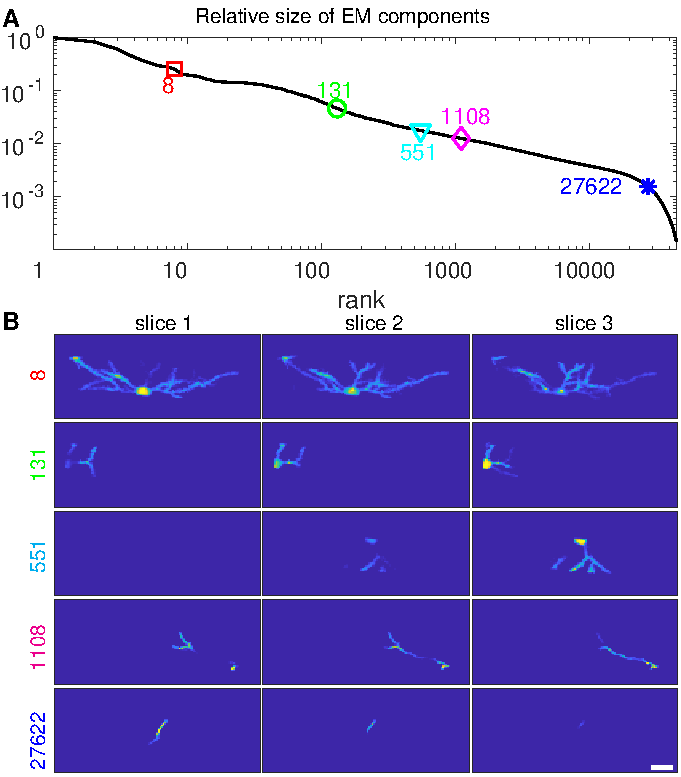
\includegraphics[width=1\textwidth]{Figs/fig_example_pi.pdf}
	\caption{Example EM footprints $\bm{p}_i$ from a single functional scan (recall that three imaging planes are obtained per functional scan in this dataset).   (\textbf{A}) The relative size (measured as the $\ell_1$ norm, $\sum_x \bm{p}_i(x)$) of the EM footprints from this scan, in decreasing order. $5$ example neurons were selected and their rank were labeled with the same color. (\textbf{B}) The spatial footprints of the 5 selected examples.  Note the wide ranges of sizes of these components; even the smallest component shown here (component 30000) could still plausibly contribute visible signal to the CI data $Y$. (Scale bar: 20 um).}
	\label{fig:em}
\end{figure}

We begin in Figure~\ref{fig:em} by examining the EM footprints $\bm{p}_i$ from a single scan.  Recall that these footprints correspond to blurred and downsampled versions of the intersection of the full three-dimensional EM segments with the imaging plane: i.e., $\bm{p}_i$ is a model of what cell $i$ would look like in a two-photon scan if the expression of the calcium indicator within the cell is uniform.

A few points are immediate.  First, there are many viable EM components visible in this scan: without any further information about cell type or calcium expression levels, there are tens of thousands of EM components with footprints $\bm{p}_i$ which could plausibly contribute signal to the CI movie $Y$.  Second, there is a wide range of footprint sizes in this dataset: when we sum over all pixels $x$, $\sum_x \bm{p}_i(x)$ varies over more than two orders magnitude from the biggest $\bm{p}_i$ to the smallest shown in Figure~\ref{fig:em}B.  Finally, it is clear that non-somatic processes (e.g.~dendrites) contribute many pixels to $\bm{p}_i$ --- in fact the large majority of pixels in the cell segments shown in Figure~\ref{fig:em}B are non-somatic, and therefore we can expect much of the signal in the CI data $Y$ to be non-somatic as well.

%EM data collected the morphological structures of all neuronal component, however, most of them were not visible in calcium imaging data due to the expression level of calcium indicators. Thus EM masks provides an over-complete set of candidate neurons for calcium imaging. 

%Figure \ref{fig:em}A shows the sorted sum ($l$-1 norm) of $\bm{p}_i$, which is the spatial footprint of the $i$- EM segments on one scanning plane of calcium imaging data. We picked $5$ example neurons and show their EM footprints (Figure \ref{fig:em}B). The spatial footprint of the $30000$-th smallest neuron can still be a potential neuronal component in calcium imaging data. 


\subsection{Initialization of single neural components}
\begin{figure}[t!]
	\centering
	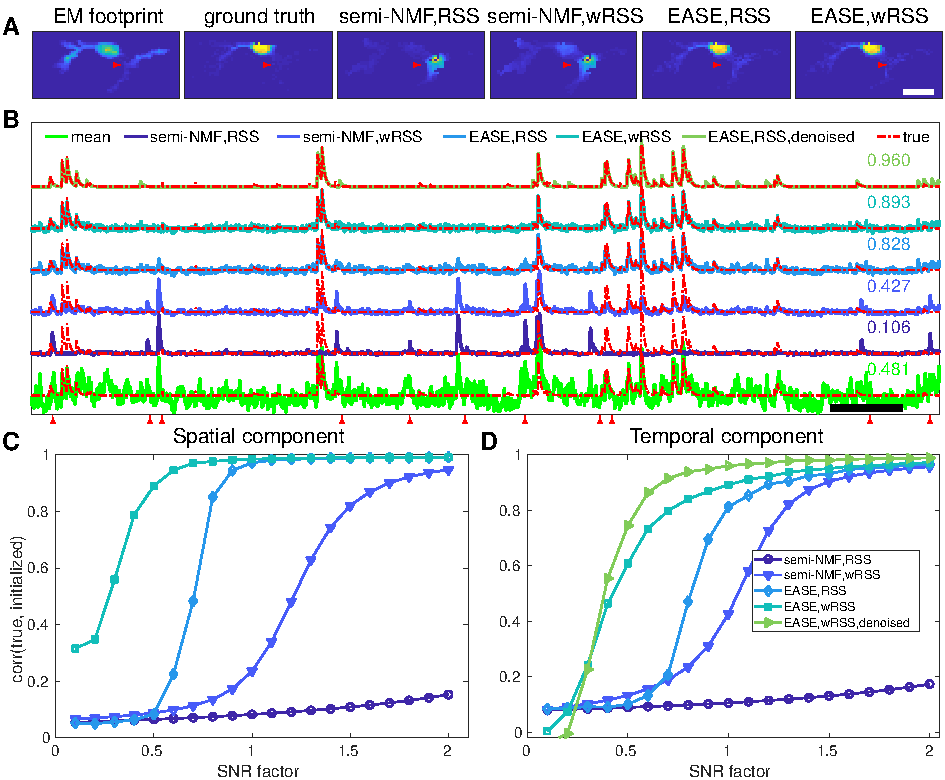
\includegraphics[width=1\textwidth]{Figs/fig_initialization.pdf}
	\caption{Comparison of different initialization algorithms.  (\textbf{A}) The ground truth and the initialized spatial footprints of the selected neuron. For simplicity, only one of the three imaging planes shown here (scale bar: 20 um). (\textbf{B}) The initialized temporal traces and their correlations with the ground-truth. %The mean trace corresponds to $\bm{z}_i$ in Eq.~(\ref{eq:z}). 
	(Scale bar: 20 seconds).  Red arrows in (\textbf{A}) and (\textbf{B}) highlight the locations or bins with large discrepancies between the estimate and ground truth. (\textbf{C} and \textbf{D}) The correlation between the ground-truth and the inferred components under different SNR levels. EASE using weighted RSS (instead of unweighted RSS) and applying denoising to the temporal trace consistently achieves the best performance in this simulation; similar results are seen when adding other ground truth components (data not shown).}
\label{fig:init_ac}
\end{figure}
% \begin{figure}[t!]
% 	\centering
% 	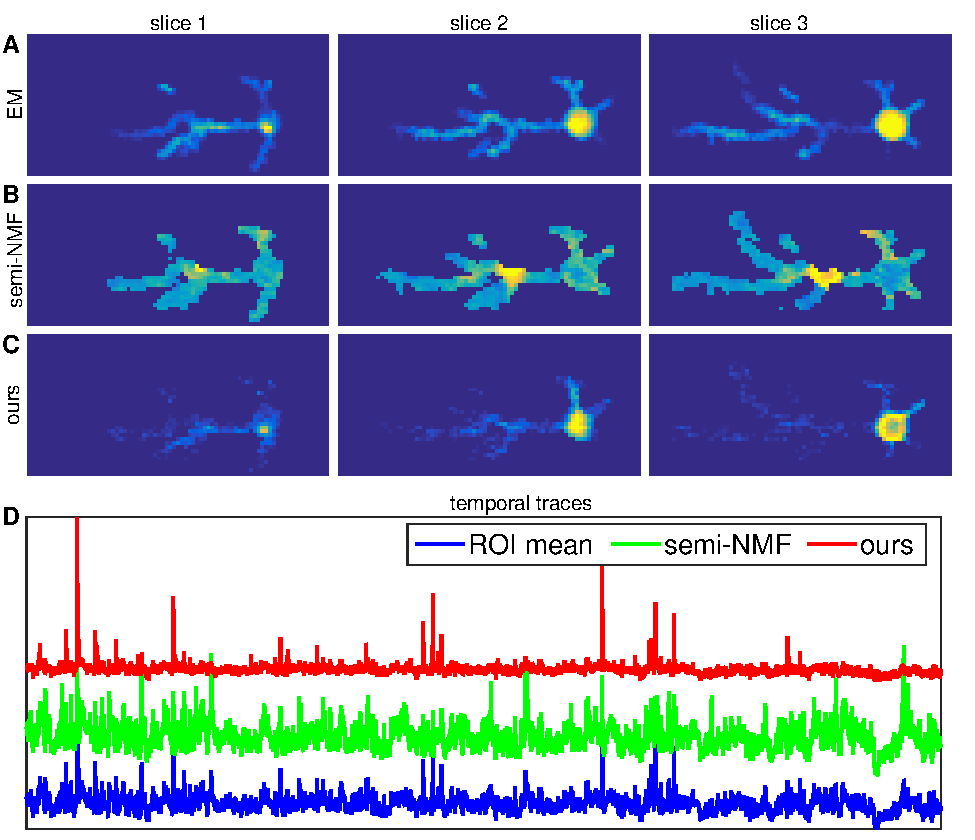
\includegraphics[width=1\textwidth]{Figs/fig_initialize_ac.pdf}
% 	\caption{Initialization of one neuron's spatial and temporal components given the EM footprint $\bm{p}_i$.  (\textbf{A}) The EM footprint $\bm{p}_i$ of the selected neuron, shown across three planes of a single scan. (\textbf{B}) initialized spatial footprint $\bm{a}_i$ of the neuron using the baseline semi-NMF approach. (\textbf{C}) same as (\textbf{B}), but using the new method proposed in section \ref{sec:init}.  Note that the EASE initialization approach outputs an initial $\bm{a}_i$ that is visually consisent with the EM footprint $\bm{p}_i$, but the semi-NMF output appears to be contaminated by signals from one or more other neurons.  \added{See also Video 2.}   (\textbf{D}) Temporal traces extracted by the EASE initialization procedure (red), the baseline semi-NMF approach (green), and by simple averaging over $\bm{p}_i$.  Note that the EASE initialization output is much sparser, because the other traces are summing over constributions of multiple cells that overlap with $\bm{p}_i$.}
% 	\label{fig:init_ac}
% \end{figure}

In section \ref{sec:init} we defined an approach for initializing functional components from the EM footprints $\bm{p}_i$, along with a simpler baseline semi-NMF method.  The main difference between these two approaches is that the EASE initialization regresses out the contribution of cells that overlap with $\bm{p}_i$ but display significant signal outside the support of $\bm{p}_i$.  We also  minimize a $\bm{p}_i$-weighted RSS (wRSS, Eq.~(\ref{eq:wRSS})), instead of the standard RSS, to further reduce nearby contaminations. We validated the necessity of these two novel contributions by simulation, where we added one neuron's spatiotemporal signal to the calcium imaging data of one scan and tried to recover this neuron's spatial and temporal components with different initialization algorithms. To make the simulation realistic and avoid confounding correlations, we generated the added neural signal from a neuron extracted from a different scan taken at a different time. Figure \ref{fig:init_ac}AB shows the comparison of different algorithms; the proposed algorithm for EASE performs the best visually. Next we varied the SNR level of the added neural signal by multiplying its temporal component by a scale factor, and quantified performance by computing the correlations between the ground-truth and the initialized results (Figure \ref{fig:init_ac}CD). Again, the proposed EASE initialization outperformed the alternative approaches consistently. %We also found that denoising the initialized traces can further recover the true signal (Figure \ref{fig:init_ac}BD). %It is also worth mention that EASE can still output a spatial footprint that is correlated with the ground truth even though the neural signal is 0 (Figure (\ref{fig:init_ac})C, SNR factor=0). Thus we remove some initializations according to the correlation between $\bm{p}_i$ and $\hat{\bm{a}}_i$.  

%In section \ref{sec:init} we defined an approach for initializing functional components from the EM footprints $\bm{p}_i$, along with a simpler baseline semi-NMF method.  The main difference between these two approaches is that the EASE initialization regresses out the contribution of cells that overlap with $\bm{p}_i$ but display significant signal outside the support of $\bm{p}_i$.  In Fig.~\ref{fig:init_ac} we see that this can make a major difference in the quality of the initialized components: the semi-NMF initialization here is contaminated  by strong background signals and at least one bright nearby neuron, yielding a spatial initialization that was very different than its EM projection (Figure \ref{fig:init_ac}B) and a temporal initialization that was likely the sum of contributions from several neurons (Figure \ref{fig:init_ac}C).  In comparison, the EASE initialization output a spatial component $\bm{a}_i$ that matched $\bm{p}_i$ closely, and a high-SNR, sparse temporal component $\bm{c}_i$.

%\added{open question - how common is this case?  does simpler semi-NMF approach work 90 percent of the time?  10?}


% 1. better than semi-nmf 
% 2. background is not a problem 
% 3. neighboring contamination is ok 
% 4. false positive doesn't yield good results 
% 5. weighing step is crucial 

%The raw data contains spatiotemporal activity of many neuronal components, thus initializing the spatial and temporal components of one neuron requires successful removal of contaminations from nearby neurons and the background. We developed a new algorithm for doing so. However, the contaminating signals may be correlated with the neuron's activity, which makes the problem hard to solve. We developed a new algorithm for solving this problem (See Materials and Methods for details). 

%As a baseline we compared against a simpler semi-NMF approach. A conventional initialization algorithm is to fit a semi-NMF model $Y_{in} = \bm{a}_i\bm{c}_i^T$ where $\bm{a}_i\geq \bm{0}$. This problem resembles problem (\ref{eq:aalpha}) except that problem (\ref{eq:aalpha}) fit the semi-NMF model for $YV_\perp$, which removes the influence of shared contaminating signals by projecting $Y$ to the null space of $V$ and highlights the unique component of $\bm{c}_i$.  The other important part of this algorithm is that the estimate $\bm{c}_i$ allows correlations with contaminating signals. These modifications are crucial for removing nearby contaminations and highlight the unique signals within the spatial support determined by EM masks. 

%\clearpage

\subsection{Extraction of neural components from a single scan}
\label{sec:one_scan}

\label{sec:example_scan}

\begin{table}
	\centering 
	\begin{tabular}{lllll}
	\toprule
	\cmidrule{1-2}
	Iteration  & add-neurons &update-model-variables  & post-processing  & \# of neurons \\
	\hline
	\hline 
	1 & $(100, 2000)$ & $ N= 1$ & - & 100\\
	\midrule
	2 & $(100, 5000)$ & $ N= 2$ & - & 175 \\
	\midrule 
	3 & $(50, 40000)$ & $ N= 3$ & fix bad matches; delete false positives& 150\\
	4 & -& $ N= 3$ & - &150 \\

	 \bottomrule
	\end{tabular}
	\caption{Details of processing pipeline steps for the example scan discussed in section \ref{sec:example_scan}. $(k_1, k_2)$ in the column \textbf{add-neurons} indicates adding $k_1$ neurons from the $k_2$ EM components with the largest L1 norm $\|\bm{p}_i\|$; \added{The actual number of the added neuron might be smaller than $k_1$ due to the quality control in Algorithm \ref{alg:initialization}. }; $N$ is the rank of the background model in Eq.~(\ref{eq:bg});% (A-m) in the column \textbf{post-processing} indicates automatically removing a neuron if its EM match does not rank within the top $m$ matches of its 2p spatial footprints among all EM segments.  (M) indicates manual deletion.  
	} 
\label{table:pipeline}	
\end{table}

\begin{figure}[t!]
	\centering
	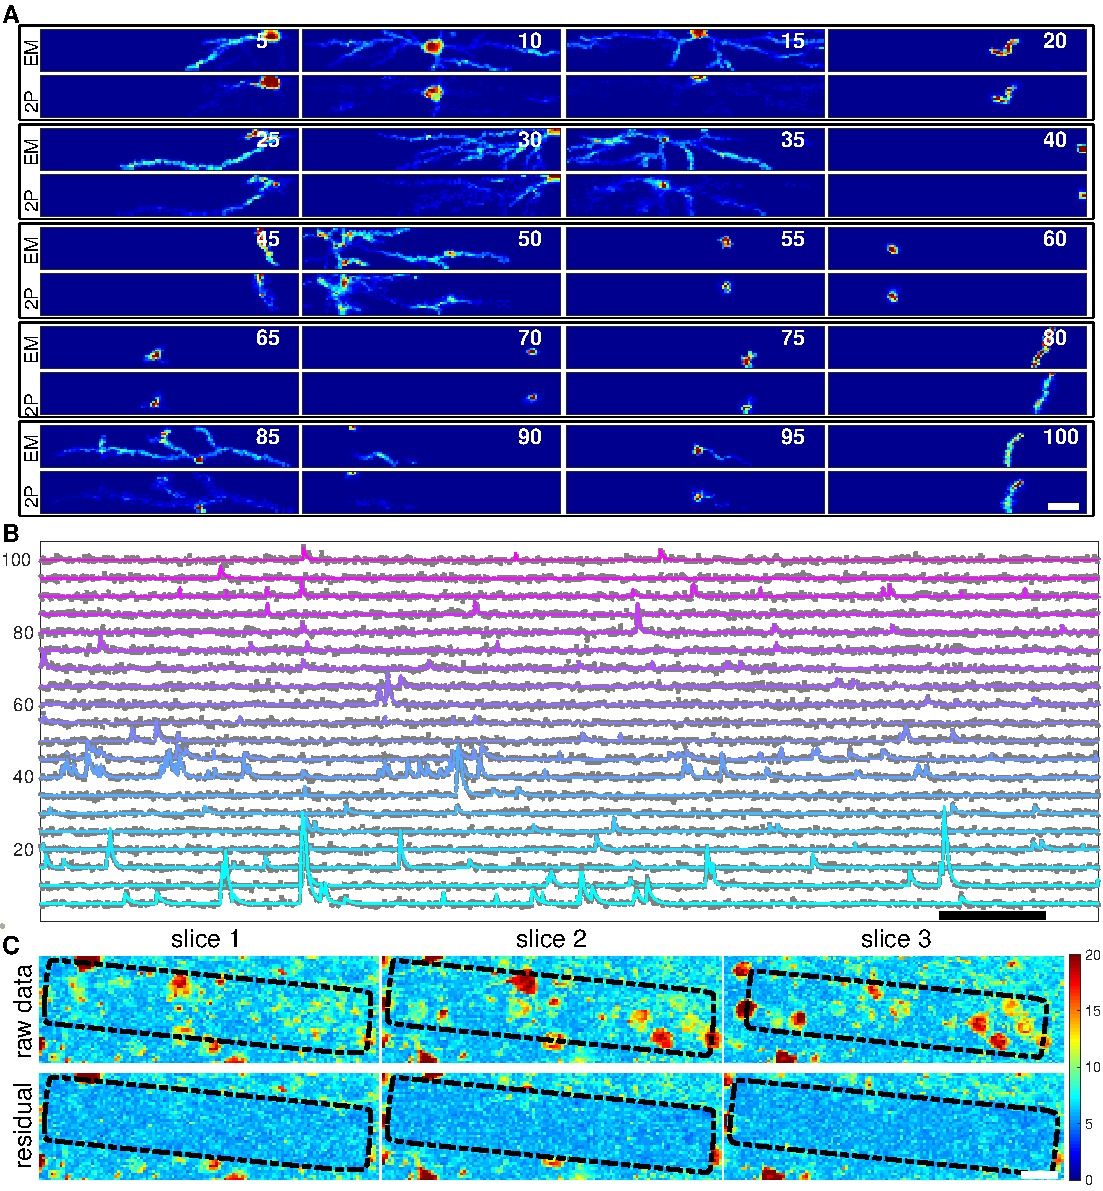
\includegraphics[width=1\textwidth]{Figs/fig_example_scan_1.pdf}
	\caption{EASE results on a single CI scan. (\textbf{A}) spatial footprints of example neurons (rank in brightness order indicated in each subpanel). Scale bar: 20 um.  Note that the EM footprints $\bm{p}_i$ and the estimated CI components $\bm{a}_i$ match each other well.  (\textbf{B}) temporal traces of the example neurons shown in A. Color traces are denoised activity; gray traces are raw.  All traces were normalized to have the same noise level. Scale bar: 10 seconds. (\textbf{C}) The peak-to-noise ratio (PNR) images before and after extracting neurons within the EM volume. Black rectangle indicates the boundaries of the EM volume;  note that no bright signals remain in the residual within this region.}
\label{fig:cn_pnr}
\end{figure}


We applied the pipeline described in algorithm (\ref{alg:pipeline}) to process data from a single scan (video size $59\times 130\times 3~ voxels \times 8900 ~frames$). The details of all iterations are summarized in Table \ref{table:pipeline}.  The automated portion of the pipeline required $\sim 10$ minutes on a desktop computer.
%The first 5 iterations required around 250 seconds. In iteration 6 and 7, we included a manual step of removing bad components and the time cost for the automatic part in these two iterations is around 200 seconds. 
The pipeline yielded $150$ components, among which an estimated $25$ components included cell bodies (identified by eye), while the remaining $125$ components included only  non-somatic processes (likely dendrites). 
Figure \ref{fig:cn_pnr}AB shows 20 example components, evenly drawn from the top 100 components (ordered by brightness). The inferred spatial CI footprints $\bm{a}_i$ resemble the corresponding EM footprints $\bm{p}_i$, as desired.  No large remaining signals were apparent upon visual examination of the residual video (\href{\videoOneURL}{S1 Video}) or the peak-to-noise (PNR) image of the residual (Figure \ref{fig:cn_pnr}C).  

In Figure \ref{fig:overlap} we examine all of the estimated spatial components $\bm{a}_i$ together.  The density of the recovered neurons is quite high, so to improve the clarity of this visualization we broke the components into five groups, sorted by the confidence scores defined in section \ref{sec:methods-joint-extraction}.  We conclude that somatic components tend to be identified with the highest confidence; then processes that branch within the field of view (leading to components $\bm{a}_i$ with a large total number of pixels); then finally, processes (including many apical dendrites) that cut through the imaging plane so that only a few pixels are visible lead to the lowest relative confidence scores.  For these components (``other," bottom row, Figure \ref{fig:overlap}) we choose not to assign a definite match, to avoid corrupting downstream analyses with an overly confident but mistaken match.

\begin{figure}[t!]
	\centering
	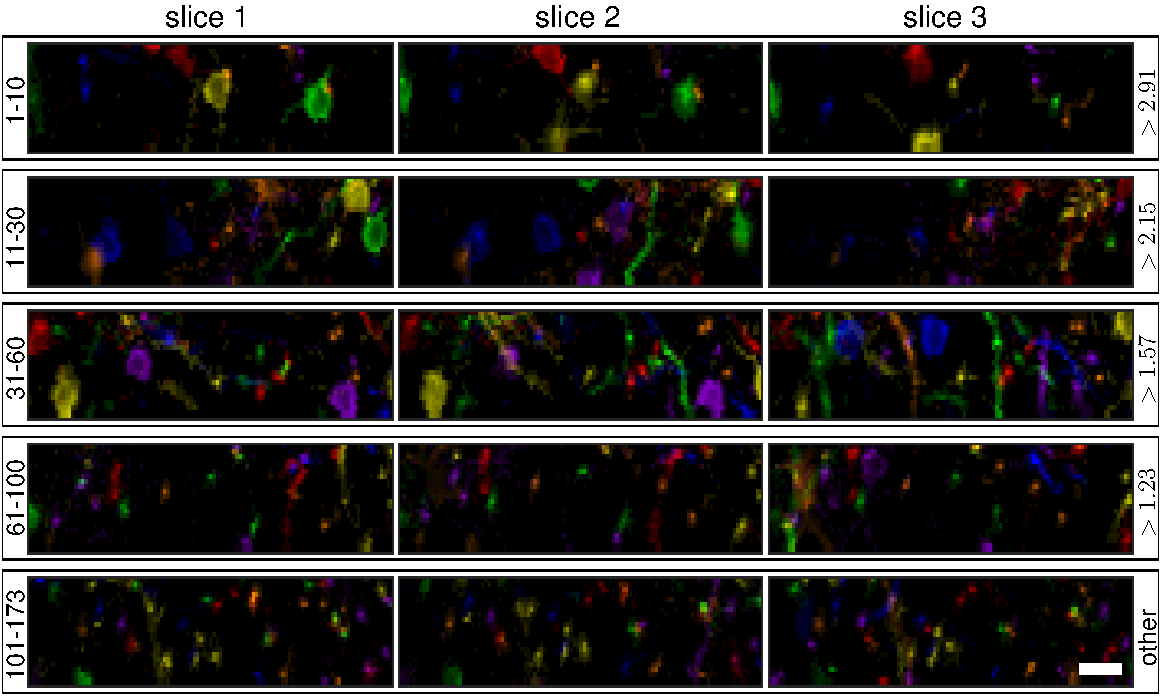
\includegraphics[width=1\textwidth]{Figs/fig_overlap_A.pdf}
	\caption{Spatial components extracted from a single scan.  Each component is indicated with a single color; the estimated $\bm{a}_i(x)$ scales the intensity of this color at each pixel $x$.  Components were ordered according to their confidence scores (defined in section \ref{sec:methods-joint-extraction}); each row here shows a subset of the spatial components $\bm{a}_i$, divided into groups according to their confidence rank (confidence ranks shown on the left; confidence score range shown on the right).  Note that confidence scores for somatic components (top rows) tend to be higher than scores for small apical dendritic components, which dominate the bottom rows here. Scale bar: 20 um. }
\label{fig:overlap}
\end{figure}


The EM information exploited by EASE provides a strong prior on the shapes of the targeted neurons, enabling the algorithm to demix neurons with strong spatial overlaps.  This point is illustrated in Figure \ref{fig:demixing}.  We performed a simple clustering to order neurons with strong spatial overlaps next to each other, leading to a strong blockwise structure in the matrix formed by computing correlations between each spatial component $\bm{a}_i$ (Figure \ref{fig:demixing}A).  Importantly, the corresponding temporal correlations (Figure \ref{fig:demixing}B) did not display the same strong blockwise structure --- i.e., components with high spatial overlap did not necessarily display correspondingly strong temporal correlations (which might have indicated problems demixing spatially overlapping signals in $Y$).  Figure \ref{fig:demixing}CD examines a block of four components with high spatial overlap: again, no problematic demixing issues are visible in either the spatial or temporal components recovered here. (See \href{\videoTwoURL}{S2 Video} for a zoomed-in depiction.) 

\begin{figure}[t!]
	\centering
	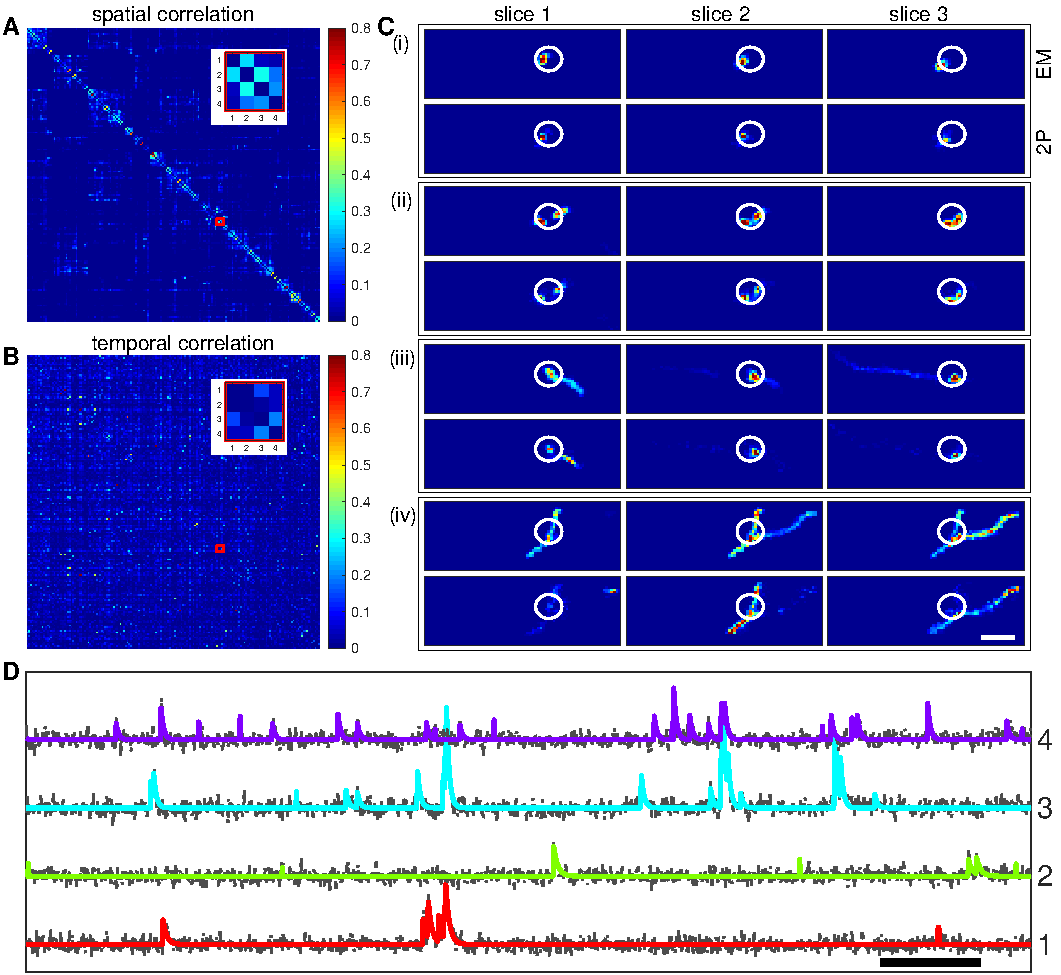
\includegraphics[width=1\textwidth]{Figs/fig_demixing_example.pdf}
	\caption{EASE can demix spatially overlapped neurons' signals. (\textbf{A}) pairwise spatial correlation between all extracted components (auto-correlations excluded to improve visibility). We used hierarchical clustering of the spatial components to place spatially overlapping neurons together.  Note the large degree of overlap visible (c.f.~Figure \ref{fig:overlap}). (\textbf{B}) pairwise temporal correlation, using the same ordering of components as in A. (\textbf{C}) spatial footprints of the selected 4 example neurons shown in the inset in panels A and B. Scale bar: 20 um.  White circles simply indicate the same location in each panel, to aid comparisons. (\textbf{D}) temporal traces of the selected neurons. Scale bar: 10 seconds. }
\label{fig:demixing}
\end{figure}


Conversely, we noticed some extracted components with highly correlated temporal traces but completely disconnected spatial components (Figure \ref{fig:merge}). By overlaying these extracted footprints onto the correlation image between the raw video $Y$ and the average of the temporal traces $\bm{c}_i$, we found that these components actually correspond to different segments of the same neuron (Figure \ref{fig:merge}A), although they were not connected within the EM volume.  These cases were rare and typically occurred at the boundary of the EM volume, where multiple dendrites from the neuron entered the EM volume at different (spatially disconnected) locations.  It would not be feasible to re-join these components with purely anatomical methods using the EM data, but the functional information from the CI data makes it possible to rejoin these severed connections with high confidence.


\begin{figure}[t!]
\centering
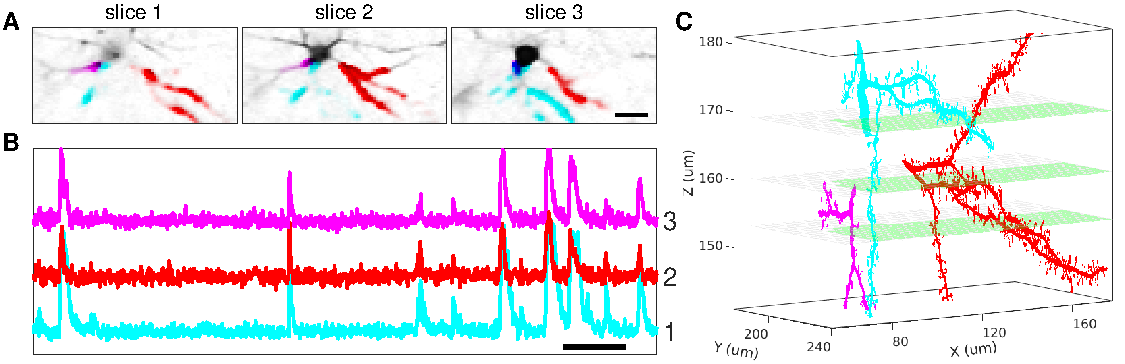
\includegraphics[width=1\textwidth]{Figs/fig_example_merge.pdf}
\caption{EASE can enable joining of split EM segments. (\textbf{A}) spatial footprints of three temporally correlated neurons (magenta, cyan, and red) and the correlation image (gray) between the raw video $Y$ and the mean of their estimated traces $\bm{c}_i$. Green rectangle indicates the boundaries of the EM volume; scale bar: 20 um. (\textbf{B}) estimated temporal components of the three selected neurons (scale bar: 10 seconds); note the strong correlation. (\textbf{C}) The EM meshes of the three neurons. } \label{fig:merge}
\end{figure}

%There is no way for the EM algorithm to reliably merge these disconnected segments, but EASE makes it possible by  fusing functional CI data and EM segments, i.e., we can bind EM segments together if their corresponding temporal traces are highly correlated. 


\subsection{Joint processing of multiple functional scans}

So far we have focused on extracting neural components from a single functional scan.  One of the major advantages of joint CI-EM data is that we can fuse information from multiple functional scans, by taking advantage of the fact that a given three-dimensional EM segment may extend over multiple scans, allowing us to match the functional signals extracted from each scan back to the same neuron.  Figure \ref{fig:multi_scan} illustrates this idea: panels A display a single three-dimensional EM segment, with the corresponding footprints $\bm{p}_i$ computed from this segment shown in panel B.  Panel C displays the functional spatial components $\bm{a}_i$ extracted from four separate functional scans, matched to the EM footprints $\bm{p}_i$ shown in panel B.  Panel D displays the corresponding temporal components $\bm{c}_i$ extracted from the four scans, and panel E shows that the visual direction tuning curve extracted from each temporal component is consistent across these scans, providing a useful secondary check on the quality of the matchings computed here.

%to come: summary figure corresponding to Figure \ref{fig:multi_scan}.  

%also another general summary figure about PNR and matching-confidence per component, number of components appearing in different scans, etc.



\begin{figure}[t!]
	\centering
	% \includegraphics[width=1\textwidth]{Figs/example_one_neuron.pdf}
	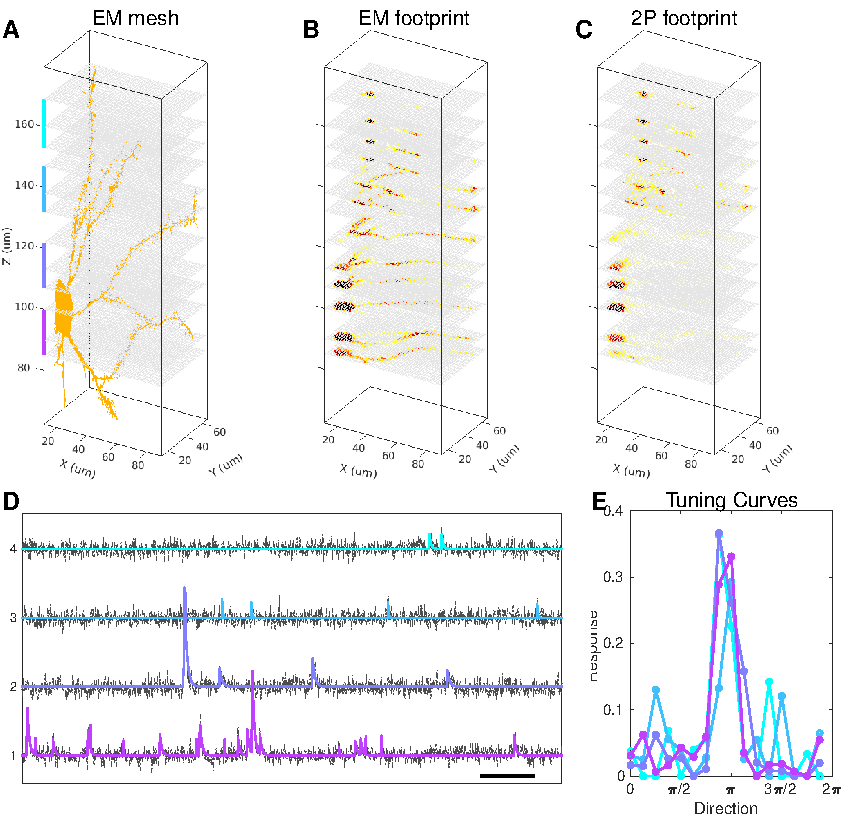
\includegraphics[width=1\textwidth]{Figs/fig_multi_scan.pdf}
	\caption{Merging the activity from a single neuron over four separate functional imaging scans.  (\textbf{A}) The extracted spatial footprints $\bm{a}_i$ of the neuron on the imaging planes of the four scans. Vertical colored bars group the three planes imaged within the same scan. (\textbf{B}) EM footprints $\bm{p}_i$ on the same imaging planes. (\textbf{C}) High-resolution EM meshes in the whole 3D volume. (\textbf{D}) The noise-normalized temporal traces $\bm{c}_i$ of this neuron imaged over the four scans (scale bar: 10 seconds).  (\textbf{E}) The direction tuning curves extracted from this neuron in each of the four scans.}
\label{fig:multi_scan}
\end{figure}
% \begin{figure}[tb]
% 	\centering
% 	% \includegraphics[width=1\textwidth]{Figs/example_one_neuron.pdf}
% 	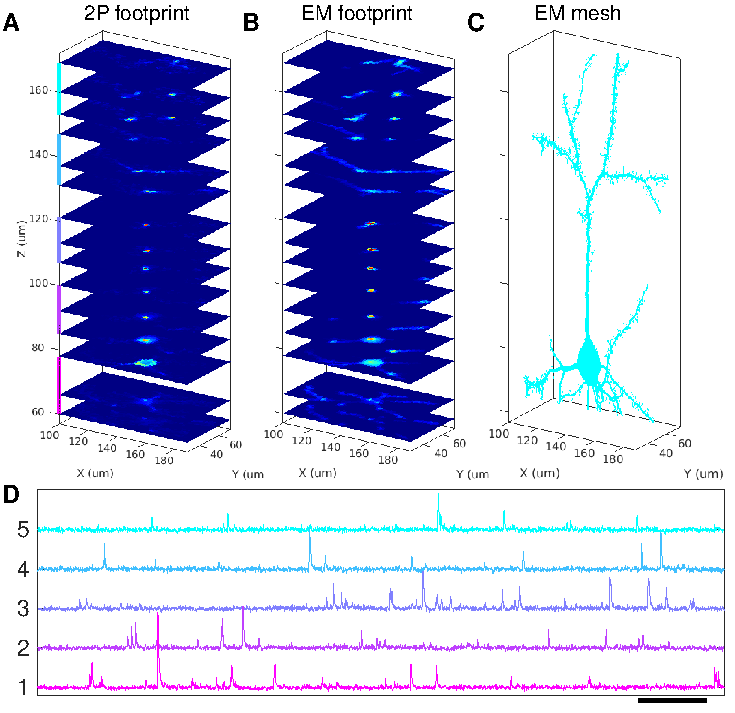
\includegraphics[width=1\textwidth]{Figs/example_1_one_in_five.pdf}
% 	\label{fig:1in5_1}
% \end{figure}
% \begin{figure}[tb]
% 	\centering
% 	% \includegraphics[width=1\textwidth]{Figs/example_one_neuron.pdf}
% 	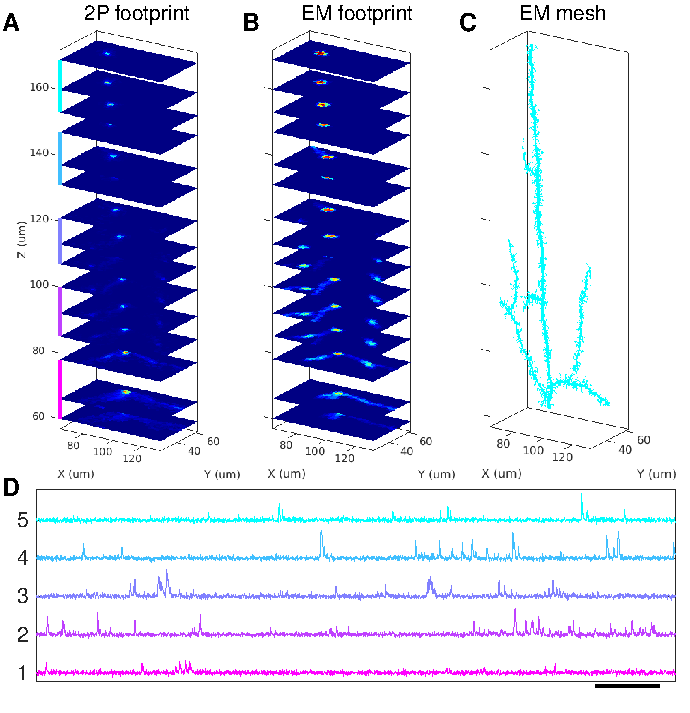
\includegraphics[width=1\textwidth]{Figs/example_2_one_in_five.pdf}
% 	\caption{Caption here}
% 	\label{fig:1in5_2}
% \end{figure}


\subsection{Comparison against constrained nonnegative factorization without EM constraints}
\label{sec:compare}

How well can CNMF methods without additional EM structural constraints recover the components extracted here?  To address this question, we ran the pipeline from \citep{Buchanan2018} on a single plane of a single functional scan, and compared the resulting spatial and temporal components to the components output by the full multi-scan EASE pipeline described above.  Figure \ref{fig:compare} compiles the results: we see that the pipeline from \citep{Buchanan2018} recovers the brightest, highest-PNR components well, but misses many dimmer components; EASE recovers about 80\% more components.  In addition, the PNR of the temporal traces recovered by EASE tends to be higher in almost all cases.  (Anecdotally, there are also cases where CNMF methods split two components that are spatially separated that can be joined using the EM prior; c.f.\ component 75 in Figure \ref{fig:cn_pnr}.)  Interestingly, we observe minimal dependence in the degree of visual tuning of the recovered components as a function of PNR, as measured by the visual direction sensitivity score described in Section \ref{sec:tc_score}.



%\added{For each extracted neuron, we found its best matched EM component by finding the one with the largest matching score (Eq. \ref{eq:score}) and then plot these largest matching scores decreasingly (Figure \ref{fig:compare}C). Clearly, the matching scores of CNMF neurons are much smaller than EASE neurons, which makes it a hard problem to reliably match CNMF neurons and EM components according to the matching scores. Actually, this is the motivation for developing this EASE pipeline. Moreover, we computed a tuning curve score (See section \ref{sec:tc_score}) to quantify how well a neuron is direction tuned. Still, the CNMF neurons has smaller tuning scores, suggesting that CNMF misses some neurons that is well tuned by direction.  }


\begin{figure}[!t]
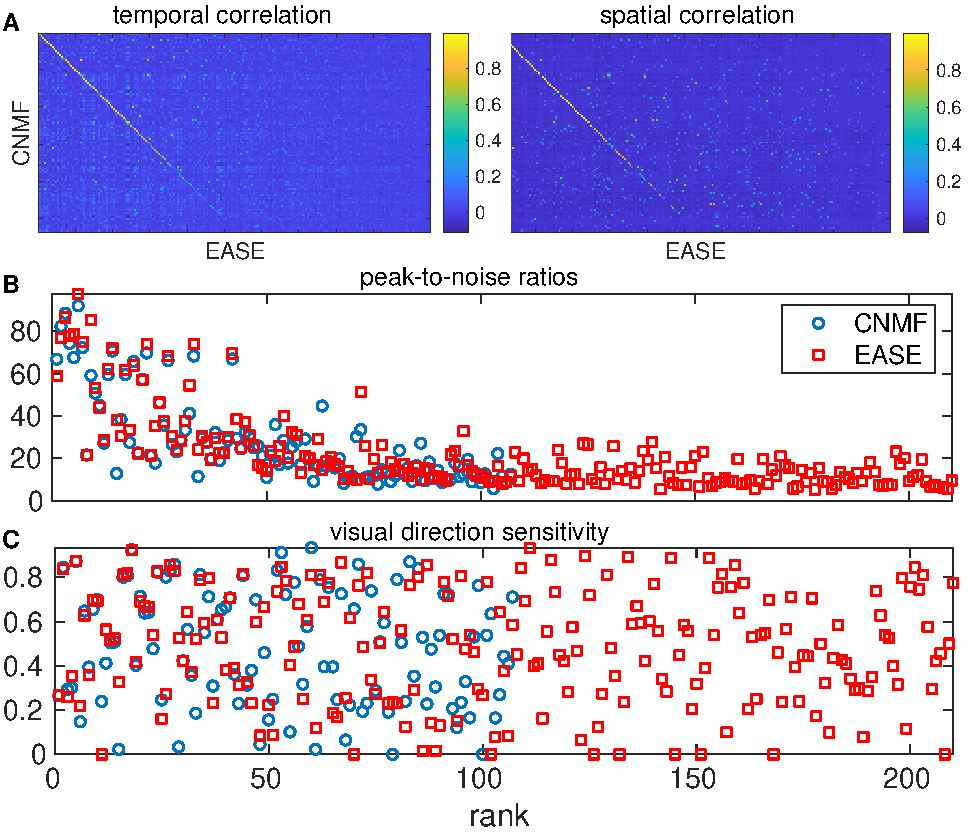
\includegraphics[width=1\textwidth]{Figs/cnmf_ease_match.pdf}
\caption{Comparison between the results of EASE and a demixing pipeline without access to EM structural prior information. (\textbf{A}) spatial and temporal pairwise correlations between neurons extracted using EASE and the CNMF-based pipeline from \citep{Buchanan2018}, respectively.  Components have been ordered to greedily maximize the diagonal of the left panel, to perform a simple matching.  EASE extracts  210 components from a single functional scan here, compared to 112 without EM structural prior information.  (\textbf{B}-\textbf{C}) PNRs (\textbf{B}) and visual direction tuning scores (\textbf{C}; Section \ref{sec:tc_score}) for all components, using the same ordering as in (\textbf{A}).  Note that EASE PNR tends to be higher than CNMF PNR, and visual direction sensitivity does not depend strongly on PNR.}
\label{fig:compare}
\end{figure}

\clearpage

\section{Conclusion}

We have introduced EASE, a method to fuse calcium imaging (CI) and electron microscopy (EM) data.  In EASE,
dense reconstruction of EM anatomy is exploited to enable dense, constrained extraction of functional CI signals.  Interestingly, in the dataset examined here, about $5 \times$ as many dendritic components as somatic components were extracted by EASE.  Thus, restricting attention to somatic components may leave significant information behind in CI recordings.  In addition, we find that EASE recovers a significant number of dim but visually-tuned components that are not recovered by standard constrained non-negative matrix factorization (CNMF) methods; thus there may be room to further improve existing CI analysis pipelines.

EASE outputs estimates of the spatial shapes and temporal activities of the neural segments visible in the field of view.  We are releasing these components publicly at \href{\resultURL}{\bf\resultURL}.  
As emphasized in \citep{Paninski2018, Soltanian2019}, we have to date lacked ground truth datasets for the CI demixing problem; since good training sets are a critical ingredient in the ``secret sauce" for accelerating progress in data science \citep{Donoho2017}, we hope that this new gold standard dataset will help accelerate development of improved algorithms for CI analysis.

Finally, it is worth noting that a version of the approach developed here should be applicable to other dense micro-anatomical approaches that are currently in development \citep{Alon2018, Gao2019}: given a three-dimensional segmentation of the anatomical channel, we can import the resulting segments, compute the footprints $\bm{p}_i$, and use these to constrain the spatial footprints $\bm{a}_i$.  We hope that these tools will enable the interrogation of dense structure-function relationships in a wide variety of neural circuits in the coming years.


\section*{Key Resources Table}


\begin{tabu} to 1\textwidth { | p{0.15\textwidth}<{\centering}| c|p{0.4\textwidth}<{\centering}| }
 \hline
 \textbf{SOFTWARE} & \textbf{LINK} & \textbf{NOTES} \\
 \hline
 EASE &https://github.com/zhoupc/ease& the implementation of the proposed pipeline \\
 \hline
 EASE\_project &https://github.com/zhoupc/ease\_project & the complete source code for reproducing this research \\
 \hline
 funimag  & https://github.com/paninski-lab/funimag  & CNMF-baselined pipeline for processing data without EM information  \\
\hline
\end{tabu}


\subsection*{Acknowledgments}

We thank E.K.\ Buchanan for useful conversations.
PZ and LP were funded by Army Research Office W911NF-12-1-0594 (MURI), the Simons Foundation Collaboration on the Global Brain, National Institutes of Health R01EB22913, R21EY027592, 1U01NS103489-01, and U19NS104649-01, NSF NeuroNex Award DBI-1707398, the Gatsby Charitable Foundation, and by the Intelligence Advanced Research Projects Activity (IARPA) via Department of Interior/ Interior Business Center (DoI/IBC) contract number D16PC00003. The funders had no role in study design, data collection and analysis, decision to publish, or preparation of the manuscript.

\subsection*{Contributions}

PZ and LP developed the EASE method and wrote the manuscript. PZ wrote the EASE software and performed all analyses described here, with supervision from LP.  DZ and IK aided in the pipeline comparisons described in Section \ref{sec:compare}.  Tolias group collected the CI data.  Allen group collected EM data.  Seung group performed EM segmentation.  JR wrangled all of the things.  \added{expand...}

\clearpage

\section{Appendix}

\subsection{Videos}

\noindent \href{\videoOneURL}{\bf S1 Video}{\bf: the demixing movie of the example data in section \ref{sec:one_scan}.} All pixel values were normalized by the standard deviation of the residual. Three columns correspond to the three planes in the selected scan.   \\

\noindent\href{\videoTwoURL}{\bf S2 Video}{\bf: the demixing movie of the 4 example neurons in Figure \ref{fig:demixing}}: The spatiotemporal signal of the extracted background and all other neuronal components except the 4 selected examples were subtracted from the raw data to construct the raw signal in this video. The video were normalized in the same way as S1 Video.  All panels use the same scaling ([-4, 4]). 


\subsection{Experimental details}
All procedures were carried out in accordance with the ethical guidelines of the National Institutes of Health and were approved by the Institutional Animal Care and Use Committee (IACUC) of Baylor College of Medicine.

\noindent{\bf Cranial Window}

Anesthesia was induced with 3\% isoflurane and maintained with 1.5\% to 2\% isoflurane during the surgical procedure. Mice were injected with 5-10 mg/kg ketoprofen subcutaneously at the start of the surgery. Anesthetized mice were placed in a stereotaxic head holder (Kopf Instruments) and their body temperature was maintained at 37C throughout the surgery using a homeothermic blanket system (Harvard Instruments). After shaving the scalp, bupivicane (0.05 cc, 0.5\%, Marcaine) was applied subcutaneously, and after 10-20 minutes an approximately 1 cm2 area of skin was removed above the skull and the underlying fascia was scraped and removed. The wound margins were sealed with a thin layer of surgical glue (VetBond, 3M), and a 13mm stainless-steel washer clamped in the headbar was attached with dental cement (Dentsply Grip Cement). At this point, the mouse was removed from the stereotax and the skull was held stationary on a small platform by means of the newly attached headbar. Using a surgical drill and HP 1/2 burr, a 3 mm craniotomy was made centered primary visual cortex (V1; 2.7mm lateral of the midline, contacting the lambda suture), and the exposed cortex was washed with ACSF (125mM NaCl, 5mM KCl, 10mM Glucose, 10mM HEPES, 2mM CaCl2, 2mM MgSO4). The cortical window was then sealed with a 3 mm coverslip (Warner Instruments), using cyanoacrylate glue (VetBond). The mouse was allowed to recover for 1-2 hours prior to the imaging session. After imaging, the washer was released from the headbar and the mouse was returned to the home cage. 

\noindent{\bf Widefield Imaging}

Prior to two-photon imaging, we acquired a low-magnification image of the 3mm craniotomy under standard illumination. The location of the subsequent two-photon field of view could then be identified in this image based on surface vasculature. The location of the target two-photon imaging site in V1 was determined by retinotopic mapping using intrinsic signal imaging or GCaMP6 imaging at low magnification.

\noindent{\bf Two-photon Imaging}

Two-photon imaging was performed in V1, in a 400 x 400 x 200 um volume with the superficial surface of the volume at the border of L1 and L2/3, approximately 100 um below the pia.Imaging data was collected with a resonant scanning microscope (ThorLabs) and software (Scanimage 5.1, Vidrio). Nine scans were collected in total, starting superficially and moving deeper into the cortex with each subsequent scan. During each 30-minute scan, a piezo controlled manipulator (PI-726, Physik Instruments) moved the microscope objective between three different z-planes (“slices”). These three slices were separated by an average of ~8 microns by the piezo, and each slice was imaged at 14.8313 frames per second. (We refer to each trio of sequential slices as a one imaging ``scan”.) Since we collected 9 scans with 3 slices/scan, we had 27 slices in total to span the 200um depth of the overall 400 x 400 x 200 um imaging volume. Two color channels were recorded: Channel one was GCaMP6 calcium imaging and channel two was blood vessels labeled with red dye (Sulfarhodamine 101). Thus each functional scan is a 256 x 256 x 2 channels x 3 slices x 27300 volume 16-bit TIFF stack. 

The mouse was head-restrained but could walk on a treadmill during imaging. While we were imaging, we collected treadmill speed at 200Hz (recorded in an HDF5 file) and we recorded a movie of the mouse’s eye at 640 x 480 @20 Hz (recorded as uncompressed .AVI). Visual stimuli were presented at 60 fps, and synchronized to imaging and behavioral data via a photodiode which recorded the timing of each stimulus frame. For each 30 minute and 40 second scan (27300 volumes at 14.8313 volumes per second) we presented 30 one-minute trials of a colored-noise stimulus \citep{niell_highly_2008} interspersed with periods of coherent motion of oriented noise. Each one minute trial contained 16 stationary-moving-stationary blocks, with a different direction presented in each block, pseudorandomly-ordered. 

To facilitate alignment with EM, at the beginning of the experiment we collected a high-resolution structural stack of the imaging volume with the same field of view and xy location as the functional scans. This stack began 310 um deep and ended at the cortical surface, in one micron steps. This stack is saved as a 512 x 512 x 2 channels x 310 slices 16-bit TIFF stack. 

\added{Add EM details here}

\subsection{Algorithm for solving (\ref{eq:opt_A})(\ref{eq:opt_C})(\ref{eq:opt_B})} \label{sec:update_abc}

There are already existing algorithms for solving the optimization problems that are the same as or similar to the subproblems (\ref{eq:opt_A})(\ref{eq:opt_C})(\ref{eq:opt_B}). We summarize the algorithms used in this work in Algorithm (\ref{alg:opt_ABC}) and briefly describe them below. 

The same problem of (\ref{eq:opt_A}) has been discussed in \citep{Friedrich2017a} and \citep{Zhou2018}. These two papers generated the spatial support of each $\bm{a}_i$ based on its previous estimation, while here we use $supp(\bm{p}_i)$ directly. The algorithm used there is modified from fastHALS \citep{Cichocki2009}. Note that the estimation of $A$ is independent of $\bm{b}_0$ because $A$ only accounts for the fluctuating signals. We estimate $\hat{A}$ first and then update $\bm{b}_0$ using the closed-form expression $\hat{\bm{b}}_0=\frac{1}{T}(Y-\hat{A}\cdot \hat{C})\cdot \bm{1}$.

\citep{Zhou2018} has a similar (\ref{eq:opt_C}) problem as here except the weighting term $\text{diag}(\sqrt{\bm{p}_i})$, thus we can reuse the algorithm by trivially including the weighting term. We iteratively update all neurons, and for each neuron we first get its unconstrained estimation 
\begin{equation}
  \hat{\bm{y}}_i = \underset{\bm{c}_i\in \mathbb{R}^T}{\text{argmin}} ~\|\text{diag}(\sqrt{\bm{p}_i}) \big(\tilde{Y}_i- \hat{\bm{a}}_i\bm{c}_i^T-\hat{\bm{b}}_0\cdot \bm{1}^T\big)\|_F^2 = \hat{\bm{c}}_i + \frac{(\hat{\bm{a}}_i\odot \bm{p}_i)^T\cdot {Y}_{\text{res}}}{(\hat{\bm{a}}_i\odot \bm{p}_i)^T\cdot\hat{\bm{a}}_i},  \label{eq:y_raw}
%   \hat{\bm{y}}_i = \underset{c_i\in \mathbb{R}^T}{\text{argmin}} ~\|\text{diag}(\sqrt{\bm{p}_i}) \big(Y-\hat{A}_{\backslash i} \cdot \hat{C}_{\backslash i} - \hat{\bm{a}}_i\bm{c}_i-\hat{\bm{b}}_0\cdot \bm{1}^T- \hat{D}\cdot\hat{F}\big)\|_F^2 = \hat{\bm{c}}_i + \frac{(\hat{\bm{a}}_i\odot \bm{p}_i)^T\cdot {Y}_{\text{res}}}{(\hat{\bm{a}}_i\odot \bm{p}_i)^T\hat{\bm{a}}_i},  \label{eq:y_raw}
\end{equation}
followed by deconvolving and denoising $\hat{\bm{y}}_i$ to infer the denoised trace $\hat{\bm{c}}_i$ and the deconvolved signal $\hat{\bm{s}}_i$ \citep{Friedrich2017b}. Once $\hat{C}$ is estimated, we also update $\bm{b}_0$ as  $\hat{\bm{b}}_0=\frac{1}{T}({Y}-\hat{A}\cdot \hat{C})\cdot \bm{1}$.

The constraint $ F\cdot \bm{1} = \bm{0}$ in (\ref{eq:opt_B}) automatically yields a closed-form estimation of $\bm{b}_0$ as  $\hat{\bm{b}}_0=\frac{1}{T}(\tilde{Y}-\hat{A}\cdot \hat{C})\cdot \bm{1}$. Then (\ref{eq:opt_B})  becomes a standard singular value decomposition (SVD) problem and the solution corresponds to the top-$N$ singular components of $\big(Y-\hat{A}\hat{C}-\hat{\bm{b}}_0\bm{1}^T\big)$. 

\begin{algorithm}[t!]
\caption{Functions for updating EASE variables}\label{alg:opt_ABC}
\begin{algorithmic}[1]
\Function{$update\_temporal$}{$Y, A, C, D, F, \bm{b}_0, P$}
% \State $Y \leftarrow Y - D\cdot F -\bm{b}_0\cdot \bm{1}^T$
\State $U \leftarrow (A\odot P)^T(Y - D\cdot F -\bm{b}_0\cdot \bm{1}^T)$ \Comment{$\odot$ is Hadamard multiplication}
\State $V \leftarrow (A\odot P)^TA$
\For{$i=1, \hdots, I$} \Comment{$I$ is the number of required iterations}
\For{$k=1, \hdots, K$} \Comment{$K$ is the number of neurons in $C$}
% \State $\bm{c}_k\leftarrow \bm{c}_k+ \frac{\bm{u}_k-\bm{v}_k\cdot C}{v_{kk}}$ \Comment{$\bm{c}_k,\bm{u}_k, \bm{v}_k$: the $k$-th \textbf{row} of $C, U, V$}
% \State $[\bm{c}_k, \bm{s}_k] \leftarrow denoise\_and\_deconvolve(\bm{c}_k)$ \Comment{$\bm{s}_k$ is the $k$-th row of S}
\State $[\bm{c}_k, \bm{s}_k] \leftarrow denoise\_and\_deconvolve(\bm{c}_k+ \frac{\bm{u}_k-\bm{v}_k\cdot C}{v_{kk}})$ \Comment{$\bm{x}_k$ indicates the $k$-th \textbf{row} of $X$}
\EndFor
\EndFor
\State $\bm{b}_0 \leftarrow mean(Y-A\cdot C) $  \Comment{average over all frames}\\
\Return $C, S, ~\bm{b}_0$
\EndFunction
\State 
\Function{$update\_spatial$}{$Y, A, C, D, F, \bm{b}_0$, P}
% \State $Y \leftarrow Y - D\cdot F -\bm{b}_0\cdot \bm{1}^T$
\State $ U \leftarrow (Y - D\cdot F -\bm{b}_0\cdot \bm{1}^T)\cdot C^T$ 
\State $V \leftarrow C\cdot C^T$
\For{$i=1, \hdots, I$} \Comment{$I$ is the number of required iterations}
\For{$k=1, \hdots, K$} \Comment{$K$ is the number of neurons in $C$}
\State $\bm{a}_k\leftarrow \max\big(0, \bm{a}_k+ \frac{\bm{u}_k-A\cdot\bm{v}_k}{v_{kk}}\big)$ \ \Comment{$\bm{x}_k$ indicates the $k$-th \textbf{column} of $X$}
% \State $\bm{a}_k\leftarrow \max\big(0, \bm{a}_k+ \frac{\bm{u}_k-A\cdot\bm{v}_k}{v_{kk}}\big)$ \ \Comment{$\bm{a}_k,\bm{u}_k, \bm{v}_k$: the $k$-th \textbf{column} of $A, U, V$}
\State $\bm{a}_k(x) \leftarrow 0 ~~ \forall x\notin supp(\bm{p}_{k^*})$ \Comment{$k^*$ is the index of the matched EM component}
% \State $supp(\bm{a}_k \leftarrow supp(\bm{p}_k$ \Comment{set $a_k(x)=0$ if }
\EndFor
\EndFor
\State $\bm{b}_0 \leftarrow mean(Y-A\cdot C) $  \Comment{average over all frames}\\
\Return $A, \bm{b}_0$
\EndFunction
\State 
\Function{$update\_background$}{$Y, A, C$}
\State $\bm{b}_0 \leftarrow mean(Y-A\cdot C) $  \Comment{average over all frames}
\State $[U, \Sigma, V] \leftarrow SVD(Y-A\cdot C-\bm{b}_0\bm{1}^T)$
\State $D=U\cdot \Sigma, F = V^T$\\
\Return $D, F, \bm{b}_0$
\EndFunction

\end{algorithmic}

\end{algorithm}

%\subsection{Details of demixing data without using EM information}
%\added{Ding, please add the details of your analysis. thanks. }

% \section{Supplementary}
% \subsection{guidance on deleting bad neurons}
% \subsubsection{automatic deletion}
% Given a extracted spatial footprint, we computed its similarity with all the EM components. If the matched EM component doesn't rank into the top k, then this neuron is deleted. 

% \subsubsection{manual deletion }
% \begin{enumerate}
% \item  spatial footprints that doesn't look like normal neurons
% \item  SNRs of the extracted traces are too low.
% \item $corr(Y, \hat{\bm{c}_i})$ is very different with $\hat{\bm{a}}_i$. This indicates that the extracted $\bm{a}_i$ may be cropped from another larger neuron. 
% \item  nearby neurons that are highly correlated. manually evaluate where some of them should be deleted. 
% \end{enumerate}


\clearpage

\bibliography{references}

\bibliographystyle{apalike}

\end{document}

\grid
